% This file (thesis-main.tex) is the main file for a master's thesis.
\documentclass {udthesis}
% preamble

% Include graphicx package for the example image used
% Use LaTeX->PDF if including graphics such as .jpg, .png or .pdf.
% Use LaTeX->PS->PDF if including graphics such as .ps or .eps
% Best practice to not specify the file extension for included images,
% so when LaTeX is building it will look for the appropriate image type.
\usepackage{graphicx}
\usepackage{cite}
\usepackage{algorithmic}
\usepackage{algorithm}
\usepackage{siunitx}
\usepackage{subscript}
\usepackage{flexisym}
\usepackage{hyperref}
\usepackage[super]{natbib}
\usepackage{subcaption}
%\usepackage{tikz}


%%% Local Variables: 
%%% mode: latex
%%% TeX-master: main.tex
%%% End: 
\DeclareSIUnit\Molar{\textsc{m}}
\DeclareSIUnit\Units{\textsc{u}}
\providecommand{\e}[1]{\ensuremath{\times 10^{#1}}}
\begin{document}
%					THESIS - TAP ( T I T L E  +  A P P R O V A L )
% 
% This is the Title and Approval Page file (thesis-tap.tex) for
% a master's thesis.
%
% The order of the commands below is very important.
% You may choose to add or eliminate a \prefacesection 
% in the front material but the order should remain 
% the same especially \maketocloflot followed by 
% \prefacesectiontoc{Abstract}

% Title and author are also used for PDF file properties
% No special character or commands can be used for the PDF definition; 
% use the [options] paramater to specify a different title or author 
% to remove special characters or commands like \\ for example.
\title[Investigating transcriptomic responses to biofuel stress in Clostridium Aceotbutylicum : Transcriptome assembly and genome annotation of a model fermentative bacterium.]{Investigating transcriptomic responses to biofuel stress in \textit{Clostridium acetobutylicum}:\\ Transcriptome assembly and genome annotation of a model fermentative bacterium.}
\author{Matthew T. Ralston}
\type{thesis}
\degree{Master of Science}
\majorfieldtrue\majorfield{Bioinformatics and Computational Biology}
\degreedate{Summer 2014}
% Optional PDF properties
\keywords{Transcriptome,RNA-seq,Assembly,Genomics}
\subject{Master of Science in Bioinformatics and Computational Biology}

\maketitlepage % Generates Title Page

\begin{approvalpage}
\prof{Eleftherios T. Papoutsakis, Ph.D.}
\chair{Errol Lloyd, Ph.D.}{Chair of the Department of Computer Science}
\dean{Babatunde Ogunnaike, Ph.D.}{Dean of the College of Engineering}
\end{approvalpage}

\begin{front} % Starts front material (Roman style page numbers)

\prefacesection{Acknowledgments}

%					A C K N O W L E D G E M E N T S
% Acknowl.tex

I write this paper with unending thanks for my family, friends, the love, support and encouragement that they give, and the lessons they have taught me. With special thanks for my mother Donna, father Thomas, and sister Allison. With special thanks to my mother; her character and duty towards others is inspirational for this work's focus on sustainability and climate change. With special thanks to my Father, for inspiration through his work ethic, leadership, and open mind. With special thanks to my sister for her support of my education, curiosity, and maturity; I would not be where I am without her encouragement and acceptance. I write this with gratitude to my family for the life they have given me, the sacrifices they have made on my behalf, and most importantly their love. With special thanks for my grandfather George inspiring my pursuit of science and chemistry. With special thanks for my grandmother Winnie for the inspiration of her love and optimism which bring me through each challenge. With special thanks for my uncle Kevin for his curiosity, friendship, optimism, and support. With special thanks for my brother-in-law Matt for his friendship and encouragement. With special thanks for my nieces Violet and Ruby for their love, for the lessons that they teach me, and their infectious energy and optimism. Many thanks for Madeline for her love, open ear, curiosity, support, and encouragement throughout the years.  Many thanks to my best friend Andrew for his friendship, curiosity, support, and encouragement. With many thanks to the rest of my wonderful and supportive family and friends for their unconditional love and support. 

Many thanks to Karol Miaskiewicz for his consistent and wonderful friendship throughout this project. Many thanks to all of the members of the Bioinformatics program. Particularly, I'd like to thank Erin Crowgey for her mentorship and support of my efforts to learn NGS bioinformatic analyses and Ryan Moore for tossing ideas around together. I'd like to thank Shawn Polson for his open ear and perspective. I'd also like to thank Dr. Wu for her support and encouragement throughout the program and the many members of the Wu group for their support as well. Many thanks to Bruce, Olga, and Summer for their work in the Sequencing and Genotyping Center in support of this project.

Many thanks for my mentors, Drs. Keerthi Venkataramanan and Terry Papoutsakis, for their mentorship, support, critique, and understanding throughout this project. The success that we've seen in this effort I owe to Keerthi's guidance and training. 
Many thanks for each of the the many members of the Papoutsakis lab for their friendship, support, and critique. I am very grateful for the unity of this group and for how much I enjoy coming to the lab each day. For the hard work, sleepless nights, early autoclave cycles, shared spaces, and plenty of reasons to celebrate I am grateful for each member.

{\centerline {\it Ad maiorem dei gloriam.}} % This file (acknowl.tex) contains the text
                % for the acknowledgments.


% Table of Contents is always created, but you
% may set \tablespagefalse and \figurespagefalse 
% if you don't want these generated automatically
% (i.e. List of Tables and List of Figures).
% These are set to true by default (i.e. \tablespagetrue,
% \figurespagetrue).

% Uncomment if you do not want a List of Figures.
%\figurespagefalse

% Uncomment if you do not want a List of Tables.
%\tablespagefalse 

\maketocloflot

\prefacesectiontoc{Abstract}

%					A B S T A C T
%% Abstract.tex


The {\it C. acetobutylicum} genome annotation has been markedly improved by integrating bioinformatic predictions with RNA sequencing(RNA-seq) data. Analysis of an initial assembly revealed errors due to technical and biological background signals, challenges with few solutions in the genomic literature. Additional hurdles for next-generation sequencing(NGS) based transcriptome mapping research include optimizing library complexity and sequencing depth, yet most studies in bacteria report low depth and ignore the effect of ribosomal RNA abundance and other sources on the effective sequencing depth. 

In this work, \textit{in vitro} and \textit{in silico} workflows were established to address false positive and negative errors associated with transcriptome mapping. An integrative analysis method was developed to integrate motif predictions, single-nucleotide resolution sequencing depth, and complexity during curation. This contextualization minimized false positive error, providing the precise and accurate determination of gene boundaries qualitifed by previous studies, in some cases, to the exact basepair. Curation of the pSOL1 megaplasmid improved statistical measures of transcriptomic features to be amenable with findings from \textit{E. coli}. 

The resulting annotation can be readily explored and downloaded through a customized genome browser, enabling future genomic and transcriptomic research in this organism. This work demonstrates the first strand-specific transcriptome assembly in the \textit{Clostridia}. Additionally, this method can be used to eliminate false positive features from assemblies in bacterial transcriptome mapping studies.  % This file (abstract.tex) contains the text
                 % for an abstract.
% Abstract.tex


The {\it C. acetobutylicum} genome annotation has been markedly improved by integrating bioinformatic predictions with RNA sequencing(RNA-seq) data. Analysis of an initial assembly revealed errors due to technical and biological background signals, challenges with few solutions in the genomic literature. Additional hurdles for next-generation sequencing(NGS) based transcriptome mapping research include optimizing library complexity and sequencing depth, yet most studies in bacteria report low depth and ignore the effect of ribosomal RNA abundance and other sources on the effective sequencing depth. 

In this work, \textit{in vitro} and \textit{in silico} workflows were established to address false positive and negative errors associated with transcriptome mapping. An integrative analysis method was developed to integrate motif predictions, single-nucleotide resolution sequencing depth, and complexity during curation. This contextualization minimized false positive error, providing the precise and accurate determination of gene boundaries qualitifed by previous studies, in some cases, to the exact basepair. Curation of the pSOL1 megaplasmid improved statistical measures of transcriptomic features to be amenable with findings from \textit{E. coli}. 

The resulting annotation can be readily explored and downloaded through a customized genome browser, enabling future genomic and transcriptomic research in this organism. This work demonstrates the first strand-specific transcriptome assembly in the \textit{Clostridia}. Additionally, this method can be used to eliminate false positive features from assemblies in bacterial transcriptome mapping studies. 

\end{front}



                   % This file (thesis-tap.tex) contains the Title
                   % and Approval Page information for a master's thesis.

%					C H A P T E R   1 - Introduction

%
% This is Chapter 1 file (chap1.tex)
%
\chapter{Title of Chapter}
This is the information for the first chapter, Chapter 1.  Copy the base file, chap1.tex, for additional chapter needed such as chap2.tex, chap3.tex, etc. Modify the main base file to include each additional chapter file.

\section{Title of Section}

This is the information for the first section of the first chapter.    % This file (introduction.tex) contains the text
                   % for Chapter 1- the introduction
                   
%					C H A P T E R    2 -  Background
% This is the file for the background chapter of my thesis

\chapter{Background}

\section{Climate Change and Renewables: A 21\textsuperscript{st} Century Challege}
Climate change research(reference) and petrochemical exploration(reference) suggest that escalated weather variation, sea levels, and atmospheric and oceanic temperatures will accompany steep increases in the cost of petroleum. Renewable chemical platforms will be an increasingly economical solution to climate change. Renewable biofuels can be carbon neutral sources of energy. Renewable biochemical processes can actually behave as carbon sinks, with net accumulation of CO_2 in chemicals and biomass after subtracting processing energy requirements.

Such a renewable biochemicals systems revolves around a biocatalyst, a microbe that can convert low cost substrates into fuels or chemicals. This production system, frequently referred to as a ``biorefinery,'' requires a microorganism with a wide range of potential feedstocks and a natural biofuel producing metabolism. Biofuels with energy density and hygroscopicity comparable to gasoline and diesel are desirable for infrastructure compatibility. The butanol-producing bacteria \textit{Clostridium acetobutylicum} consumes a number of sugars and hydrolysates and produces a direct gasoline replacement (citation).

\textit{C. acetobutylicum} is a historically industrial solvent producer(reference Weizmann review). It consumes lignocellulose (source), a variety of simple and complex carbohydrates, and hydrolysates. Also known as the Weizmann organism, \textit{C. acetobutylicum} converts these substrates into solvents through an acetone, butanol, and ethanol (ABE) fermentation.  Importantly, these cells synthesize most amino acids with ammonium salts as a nitrogen source, requiring only a minimal defined medium. This microbe meets the requirements for low-cost non-food feedstocks and infrastructure compatibility. Therefore, \textit{C. acetobutylicum} is an excellent chassis organism for an integrated biorefinery and is the system of study in this work.

\textit{C. acetobutylicum} has a number of intrinsic advantages that minimize the engineering efforts required for bioprocess development. It is one of over 17,000 bacteria with sequenced genomes\cite{89,90,91} and has a substantial research community(cite clostridial conference paper?). For example, current metabolic models (cite Maciek's article) are used for sophisticated metabolic analyses, such as $C_{13}$ metabolic flux analysis. A model for the solventogenic \textit{Clostridia}, \textit{C. acetobutylicum} is a reasonably well studied organism with industrial potential.

Prior to the genomic era, targeted studies in this organism revealed the specific loci for solvent formation(references), sporulation(references), and some heat-shock genes(references). These genes were typically cloned, sequenced, and  investigated with gene-specific transcriptomic techniques. However, only the mechanisms of the unique metabolic systems (e.g. solvent formation) have been investigated in detail; The mechanisms for the majority of the genetic and metabolic systems in \textit{C. acetobutylicum} are largely inferred from homology and often, this assumption is appropriate. 

That being said, many of the most interesting characteristics of \textit{C. acetobutylicum} are unique to the \textit{Clostridia}. Of particular interest for biosystems engineering is its solvent stress-response, which may be uniquely adapted to biofuels. A number of stress-response systems exist for specific stresses, with broader systems that respond to multiple stressors. The knowledge of these systems reflects the knowledge of the \textit{C. acetobutylicum} genome generally. In the next section, stress-response systems are reviewed, demonstrating opportunities for the discovery of novel transcriptomic features.

\section{Biofuel/Solvent Tolerance and the Bacterial Stress Response}


%          REARRANGE ME!!!

Optimizing \textit{C. acetobutylicum} strains for bioprocesses requires detailed knowledge of their metabolic and genetic networks. While quality metabolic reconstructions have been described (reference Keerthi/Antoniewicz paper), its genetic networks are less complete and largely rely on bioinformatic inferences without experimental evidence. One such genetic system concerns solvent tolerance and stress response systems, as hydrophobic and amphipathic biofuels negatively affect cell viability and survival. These systems are essential for the development of solventogenic bioprocesses. As we will see, knowledge of the \textit{C. acetobutylicum} stress response is far complete, due in part to an incomplete genome annotation. Next, these stress-response systems and the extend of their knowledge in \textit{C. acetobutylicum} are briefly reviewed.


Unfortunately, the \textit{C. acetobutylicum} stress response network was poorly defined. As of April 2014, Over 17,000 bacterial genomes have been sequenced\cite{89,90}, including \textit{C. acetobutylicum}\cite{91}. Initial bioinformatic analysis of the \textit{C. acetobutylicum} genome predicted just under 4,000 genes, including some canonical genes of the stress response\cite{91}. Most of the genes lacked experimental evidence and most early efforts have revolved around heat-shock systems.

Unfortunately, gene-specific characterization is both difficult and time consuming. Therefore, a genome-wide technique was desired to identify candidates for further investigation. 

Both specific and general stress response systems are useful for biosystems engineering.
%          REARRANGE ME!!!

Bacteria respond to a wide variety of intrinsic and extrinsic challenges with stress response systems. For example, nutrient deprivation, osmotic shock, temperature fluctuation, and high chemical concentrations are common in their natural environments. Cells activate specific or general response networks after these insults. \textit{C. acetobutylicum} is a naturally solventogenic bacterial species and could possess solvent-tolerance genes that would likely be regulated by general or specific stress response systems. Such genes would be natural targets for biosystems engineering, improving the tolerance of engineered strains to high biofuel titers. 

Unfortunately, knowledge of these systems is incomplete in \textit{C. acetobutylicum} and no unique solvent tolerance genes, such as solvent exporters, have been identified. The stress response is an important system for biotechnology, but the annotations of \textit{Clostridia} genomes require improvement for understanding of these and other systems. Here we review these systems and the extent of their knowledge in \textit{C. acetobutylicum}.


\subsubsection{Specific Stress Response Systems}
Specific stress-responses are designed to mitigate the negative effects of a particular stressor. These systems typically contain a detection mechanism for either the stressor or its effects, such as antibiotics or DNA damage, respectively.

Antibiotic resistance is an example of a specific stress response system that can detect a molecular stressor. In the presence of organic compounds of the $\beta$-lactam, tetracycline, and (others?) families, bacteria activate antibiotic resistance genes that either export or modify the organic compounds to prevent their action (review reference). Some of these antibiotic-resistance genes are part of operons that possess antibiotic-detecting repressors (review citations). Upon the detection of the antibiotic agent, a confirmation change triggers derepression of the antibiotic resistance gene and subsequently an antibiotic resistant phenotype. This stress response system helps the bacteria respond quickly and specifically to compounds from a family of antibiotics, but typically do not confer survival benefits to other stressors, such as heat stress.

A second example of a specific stress response is from \textit{D. radiodurans}, which has an unparalleled resistance to ionizing radiation (reference). In response to breaks in DNA, \textit{D. radiodurans} repairs the multiple copies of its genome, enabling growth, viability, and survival at over 5,000 Gy of radition (reference). This system responds instead to the symptom of $\gamma$-radiation, DNA damage. The extreme tolerance of \textit{D. radiodurans} to radiation is a byproduct of a specialized system for DNA repair, augmented from the standard DNA repair system. This system contains a detection system, non-homologous recombination, and a specialized DNA repair system allows \textit{D. radiodurans} cells to survive and repair hundreds of insults to its genome. 

If specific stress response systems exist for solvent stress (e.g. solvent exporters), they would be desirable targets for research in solventogenic \textit{C. acetobutylicum}. Stress responsive small RNAs have been described(Keerthi's small RNA paper), although their roles, regulation, and conservation remain unknown. To identify genes that could serve this role, differential expression experiments are desirable. The statistical treatment of measurements for such experiments is complex and requires reliable estimates of transcript expression. These estimates would be difficult to acquire with the original bioinformatically-predicted genome annotation. An improved genome annotation could yield novel stress-responsive transcripts and improve expression estimates by counting reads at the transcript level, as opposed to the ORF level.

In addition, an improved genome annotation complete with transcription start sites and regulatory regions would facilitate research on the regulation of a hypothetical specific solvent stress-response system. Regulatory motifs can be discovered with enrichment methods (RSAT reference) with a complete set of transcript boundaries. Regulatory networks are targets for engineering purposes but difficult to research, especially without precise knowledge of gene boundaries.

The first type of stress-response system reviewed can have unique detection and response mechanisms to specific intrinsic or extrinsic stressors. These genes have important applications in environmental remediation (D. raiodurans cleanup), pharmaceutical research (antibiotic research, tier design), and more. The next stress-response systems reviewed respond to more than one stressor, conferring a more general survival benefit.


\subsubsection{General Stress Response Systems}

In contrast to specific stress-response systems, general responses are activated by more than one stimulus. These programs provide non-specific survival benefits to more than one stressor. For example, during both nutrient deprivation and acid stress, cells must slow or cease growth (stringent response) to adapt to energetic demands of the activation of both the specific and general stress response program. Also, both heat-shock(citation) and solvent stress(citation) can denature proteins and consequently activate chaperonin systems, another example of a general stress response. After detection of the stressor, signal transduction events activate dormant response machinery (citation) or activate/derepress response systems(citation). The general stress response is divided into four classes of genes based on the regulator responsible for their activation. 

\paragraph{Class I}
The first class of general stress response genes is governed by the repressor HrcA, which responds to protein denaturation from thermal or chemical causes. The HrcA regulon contains at least 3 transcripts including the HrcA and DnaK/J, GroES/EL, and htpG loci(Qinghua, other citations). Denatured proteins titrate the groEL chaperone from HrcA/groEL complexes, resulting in a conformational change of HrcA and decreased DNA binding(source). Operons regulated by the HrcA repressor are subsequently derepressed, rapidly increasing the amount of heat shock proteins. Protein denaturation negatively affects nearly every program and structure of the cell, resulting in decreased survival and viability. In \textit{C. acetobutylicum}, the HrcA motif was recently described(citation) for standard heat-shock operons. Additionally, class I genes are solvent-stress responsive (citation) due to solvent-induced protein denaturation. It is unknown if any additional operons are also regulated by this repressor in \textit{C. acetobutylicum}. To answer this question, an improved genome annotation including transcription start sites would facilitate the discovery of additional genes in the HrcA regulon through \textit{in silico} analyses.

\paragraph{Class II}
The second class of genes is regulated by a stress-responsive $\sigma$-factor, $\sigma$_{B}. In \textit{B. subtilis}, the $\sigma$_B regulon consists of ___ genes and coordinates a general stress response for a variety of stressors. A \textit{C. acetobutylicum} $\sigma$_B ortholog was not predicted in the initial genome annotation, although the various stress response genes (HrcA under Sig B regulon CITATION) remain. The regulation of these genes is unknown in this organism. Perhaps $\sigma$_{B} genes in \textit{C. acetobutylicum} are under the control of an overlapping regulon, as in \textit{L. monocytogenes}. Given the large size of the $\sigma$_B regulon and the presence of several of its genes (e.g. HrcA(citation), clpC), the promoter and regulatory regions of \textit{C. acetobutylicum} orthologs of $\sigma$_{B} regulon genes would be useful for understanding the unique stress response of \textit{C. acetobutylicum}. This class of general stress-response genes present another opportunity for an improved genome annotation to facilitate stress response research.

\paragraph{Class III}
The third class of genes is regulated by the repressor CtsR, with a ____ transcript regulon in \textit{B. subtilis}. CtsR is a dimeric helix-turn-helix regulator that is capable of responding to heat-shock, oxidative stress, and acid stress(references from lit review of CtsR-thiol paper). In \textit{B. subtilis}, CtsR responds to heat-shock when clpC, the fourth gene of the CtsR operon, releases McsB(reference). Free McsB phosphorylates CtsR, leading to positive autoregulation and derpression of the CtsR regulon. This mechanism is thought to vary across the gram positive bacteria(reference), but the operon organization suggests that the \textit{C. acetobutylicum} CtsR system is similar to \textit{B. subtilis}(Qinghua paper). A CtsR motif was found ahead of canonical CtsR regulon genes in \textit{C. acetobutylicum}(Qinghua paper) although additional genes may be controlled by CtsR in the absence of $\sigma$_{B}. A genome-wide motif search in this organism could similarly reveal CtsR regulation of solvent responsive transcripts. Similar to the class I system, knowledge of the CtsR regulon would also benefit from an improved genome annotation.

\paragraph{Class IV}
The fourth and final class of general stress-response genes are regulated by unknown mechanisms. In \textit{C. acetobutylicuM}, this class includes stress-responsive genes with unconfirmed operon structure and no confirmed motifs. Microarray experiments from Venkataramanan show over 1,000 solvent responsive genes in \textit{C. acetobutylicum}, the regulation of which remains almost completely unknown. As suggested above, an improved genome annotation would aid the categorization of this massive gene set into class I, III, or potentially new regulons.

These general stress response programs are vital for adaptation and robustness. However, both sporulation and stress-response systems in the \textit{Clostridia} differ from the model for sporulating gram positive bacteria, \textit{B. subtilis} (Pap sporulation review). At the very least, specific regulatory genes are missing such as the sporulation regulator ____ (Pap sporulation review) and the stress response regulator $\sigma$_B. Furthermore, most solvent responsive genes in \textit{C. acetobutylicum} are regulated by unknown motifs and response regulators. Finally, it is reasonable to expect that there may be some stress-response genes specific to the solventogenic \textit{Clostridia}, perhaps even exclusively solvent responsive. Such genes would have had little homology to known genes during the initial genome annotation and therefore would not be included in previous comparative genomic and microarray analyses. For example, a recent study identified unique solvent responsive small RNAs in \textit{C. acetobutylicum}, many with no known homologs or regulators (keerthi small RNA). Clearly, there is much to be done to understand and develop this organism for biofuel applications.

In this section, the example of stress-response systems was used to demonstrate differences of \textit{Clostridia} from the \textit{Bacillus} model. Also, it is clear that with current knowledge of the \textit{C. acetobutylicum} genome, there are opportunities to discover novel transcripts or proteins not described by the initial genome annotation and provide precise transcript boundaries for motif identification. In fact, the current annotation relies almost entirely on bioinformatic ORF predictions. To provide definition to the stress response and other systems, regulatory regions and operon organization should be revealed by modern transcriptomic techniques. Next, techniques that provide these details throughout the genome are discussed.

\section{Transcriptomic Research}
Modern high-throughput techniques can produce genome-wide data, even when reference genomes are not available (de novo assembly reference, metatranscriptomics). An enormous number of array and sequencing techniques have been developed to investigate the proteome, transcriptome, and interactome including protein-protein(Chang Tse-Wen), protein-DNA(chip on chip, ChIP-seq), protein-RNA(pulldown, and RNA-RNA interactions (microRNA array, HITS-clip), protein post-translational modifications, single nucleotide polymorphisms, and transcript expression(Mark Schena microarray, RNAseq). In this section, transcriptomic techniques are reviewed and experimental designs discussed for this study's objective of revealing transcript boundaries, regulatory regions, and operon organization.

\subsection{Experimental Designs}
Transcriptomic techniques allow the characterization of the properties and dynamics of RNA species. In the last decade, microarrays and sequencing techniques have revolutionized transcriptomic research, providing new insights into the complexity of the transcriptome (E. coli sRNA, miRNome, ncRNAs, snoRNAs etc) and its regulation(HFQ, Argonaute, turnover). Understanding of this dynamic population is just beginning, in addition to its interactions with the metabolome(riboswitch) and proteome(HFQ, regulatory proteins) levels. Two common experimental objectives are used to explore cellular programs: annotation and differential expression.

\subsubsection{Genome Annotation}
Before differential expression experiments are conducted, or in instances where a complete genome is not available, the catalog of all genes and their transcripts is required for microarray probe design or sequence read counting. ORF prediction algorithms(Glimmer citation, AUGUSTUS) and annotation suites(RAST citation, MG-RAST citation) can identify putative ORFs encoding enzymes and canonical genes for sequenced genomes. However, unique genes and small RNAs cannot be identified with these predictions. It is desirable to experimentally determine the transcriptome for conditions of interest.

Tiling microarrays(Bsub) and deep RNA sequencing(one of the strand specific papers) can be used to identify novel transcripts, transcript boundaries, and operon organization. Strand specific options for these methods are especially useful in dense bacterial genomes. Computationally, type I and II errors make automation of transcript annotation difficult without making assumptions. Nevertheless, transcriptome assembly methods permit the reconstruction of full-length transcripts from sufficiently deep sequencing datasets.

By assembling a complete catalog of transcripts, novel transcripts and regulatory RNAs can be identified for further analyses. Also, a transcriptome assembly is useful in instances where a complete genome sequence is unavailable. The transcripts can also be annotated for ORFs, with the benefit of experimental evidence and Shine-Dalgarno motifs. Finally, a complete catalog of transcripts is useful for obtaining accurate estimates of gene expression and understanding coexpression patterns.

\subsubsection{Differential Expression}


\subsection{Analytical Methods}

\subsubsection{Microarray}

\subsubsection{RNA Sequencing}




%					C H A P T E R   2 - Methods
% This is the Chapter 2 - Methods file (chap2.tex)

\chapter{Methods}


\section{Culture}
Wild type \textit{Clostridium acetobutylicum} ATCC 824 was cultured anaerobically in 4L New Brunswick Scientific BioFlo 310 bioreactors at \SI{37}{\degreeCelsius}, pH >5.0, \SI{200}{\milli\liter\per\minute} N\textsubscript{2} and 200rpm agitation in a defined \textit{Clostridia} growth medium, as described previously (Venkataramanan 2013). When the cultures were grown to A\textsubscript{600}=1, the N\textsubscript{2} flow rate was decreased to \SI{50}{\milli\liter\per\minute} and cultures were either stressed to a final concentration of \SI{60}{\milli\Molar} \textit{n}-butanol, \SI{40}{\milli\Molar} potassium butyrate, or left unstressed. \SI{15}{\milli\liter} samples were acquired at 15, 75, 150, and 270 minutes after treatment and synchronization. Samples were centrifuged at 8,000rpm, \SI{4}{\degreeCelsius} for 20 minutes. After discarding the supernatant, cell pellets were then immediately frozen at \SI{-85}{\degreeCelsius}.

\section{RNA preparation}
RNA was extracted by first washing the cell pellets in 1mL of RNase-free SET buffer (25\% sucrose, \SI{50}{\milli\Molar} EDTA [pH 8.0], \SI{50}{\milli\Molar} Tris-HCl [pH 8.0]) before resuspending cells in a \SI{220}{\milli\liter} solution of RNase-free SET buffer containing \SI{4.55}{\Units\per\milli\liter} proteinase K and \SI{20}{\milli\gram\per\milli\liter} lysozyme and incubating for 6 minutes. Resuspended cells were vortexed with 40mg of RNase-free glass beads ($\leq$\SI{106}{\micro\metre}) at maximum speed and room temperature for 4 minutes. Each sample was mixed immediately with \SI{1}{\milli\liter} of ice-cold QIAzol (Qiagen, Valencia, CA, USA) and then \SI{200}{\micro\liter} of ice-cold chloroform, mixing well. After a 3 minute room temperature incubation, samples were centrifuged at 11,000rpm and \SI{4}{\degreeCelsius} for 15 minutes. The aqueous phase was then mixed with \SI{1.3}{\milli\liter} of ice-cold ethanol before transfering to a miRNeasy Mini spin-column (Qiagen, Valencia, CA, USA) and centrifuging at 11,000rpm and \SI{4}{\degreeCelsius} for 15 seconds.

Next, \SI{700}{\micro\liter} of RWT buffer was added to the column, before centrifuging at 11,000rpm and \SI{4}{\degreeCelsius} for 15 seconds, discarding the collection tube and transferring the column to a fresh collection tube. The column was washed twice with \SI{500}{\micro\liter} of RPE buffer before centrifuging at 11,000rpm and \SI{4}{degreeCelsius} for 15 seconds each. The membrane was then dried with an additional centrifugation step at 11,000rpm and \SI{4}{degreeCelsius} for 1 minute. The RNA was eluted twice by incubating with \SI{50}{\micro\liter} of nuclease-free water for 1 minute and eluting for 1 minute at 11,000rpm and \SI{4}{degreeCelsius}.

After quantification on a Nanodrop ND-1000, samples were then precipitated in 0.3M sodium acetate and 75\% ethanol overnight, centrifuged at 14,000 rpm for 30 minutes, washed twice with \SI{400}{\micro\liter} ice-cold 70\% ethanol, and rehydrated in \SI{50}{\micro\liter} RNase-free water. Next, samples were treated with the Turbo DNA-free kit (Ambion, Austin, TX, USA). \SI{5}{\micro\liter} of 10X Turbo DNase buffer and \SI{1}{\micro\liter} of Turbo DNase (2U\SI{}{\per\micro\liter}) were added to each sample before incubating at \SI{37}{degreeCelsius} for 30 minutes. Next, \SI{5}{\micro\liter} of DNase inactivation reagent were added to each sample, mixing occasionally for 5 minutes. The samples were then centrifuged at 10,000rpm and \SI{4}{degreeCelsius} for 90 seconds, precipitating the DNase. 

Samples were then precipitated, washed twice more with 70\% ethanol, and resuspended in \SI{20}{\micro\liter} of nuclease-free water, requantified, and aliquoted for quality analysis with the BioAnalyzer platform (Agilent, Wilmington, DE, USA), and \SI{10}{\micro\gram} aliquots in \SI{10}{\micro\liter} samples were stored at \SI{-85}{\degreeCelsius}.

\section{RNA enrichment, RNA-seq library preparation, and Sequencing}
Ribosomal RNA was removed with the MicrobExpress kit (Ambion, Austin, TX, USA) according to their protocol. Briefly, beads were prepared by taking \SI{50}{\micro\liter} for each sample, washing with an equal volume (\SI{50}{\micro\liter}) of water capturing for 5 minutes on a MagnaSphere (Promega, Madison, WI, USA) magnetic stand and aspirating. Subsequently, the beads were resuspended in an equal volume (\SI{50}{\micro\liter} each) of binding buffer and capturing as above. The beads were then resuspended in an equal volume (\SI{50}{\micro\liter} each) of binding buffer and warmed to \SI{37}{\degreeCelsius}. Next, \SI{200}{\micro\liter} of binding buffer was added to each \SI{10}{\micro\gram} RNA aliquot with \SI{4}{\micro\liter} of capture oligo mix. The mixture was warmed to \SI{70}{\degreeCelsius} for 10 minutes, then cooled to \SI{37}{\degreeCelsius} for 15 minutes. Next, the rRNA was captured by mixing \SI{50}{\micro\liter} of beads with each sample, incubating for 15 minutes at \SI{37}{\degreeCelsius}, and capturing as above. The enriched RNA was transferred to a fresh \SI{1.5}{\milli\liter} tube. The beads were then washed with \SI{100}{\micro\liter} of pre-warmed (\SI{37}{\degreeCelsius}) wash solution, incubating on the magnetic stand for 5 minutes, and adding the wash solution to the enriched RNA. The samples were then ethanol precipitated at \SI{20}{\degreeCelsius} overnight with \SI{35}{\micro\liter} of \SI{3}{\Molar} Sodium Acetate, \SI{5}{\milli\gram\per\milli\liter} Glycogen, and \SI{1175}{\micro\liter} of chilled 100\% ethanol. The samples were washed twice with 70\% ethanol and resuspended in \SI{25}{\micro\liter}. The samples were enriched further by repeating the MicrobExpress treatment. Small 10-\SI{100}{\nano\gram} aliquots were analyzed at each step with the BioAnalyzer to monitor enrichment.

Selected samples were enriched further with Terminator 5'-phosphate dependent exonuclease kit (Epicentre, Madison, WI, USA). Terminator Exonuclease \SI{1}{\micro\liter} (1U\SI{}{\per\micro\liter}) was added with \SI{2}{\micro\liter} 10X Buffer A to each RNA sample. The reaction was run in a      thermocycler for 60 minutes at \SI{30}{\degreeCelsius}. The reaction was terminated with the addition of \SI{1}{\micro\liter} of \SI{100}{\milli\Molar} EDTA and ____ Tris HCl at pH 8.0. The samples were then purified by ethanol precipitation (\SI{0.3}{\Molar} Sodium Acetate and 75\% ethanol) with two 70\% ethanol washes, as above.
Enriched RNA was quantified as above and assessed for quality with the BioAnalyzer platform (Agilent, Wilmington, DE, USA). High quality samples were used to prepare RNA-seq libraries with the ScriptSeq v2 library preparation kit and indexed PCR primers (Epicentre, Madison, WI, USA). Briefly,  \SI{1}{\micro\liter} of fragmentation solution and \SI{2}{\micro\liter} of cDNA synthesis primer was added to \SI{50}{\nano\gram} of RNA and the solution was fragmented for 5 minutes at \SI{85}{\degreeCelsius} in a _____ thermocycler. To each reaction, \SI{0.5}{\milli\Molar} of Dithiothreitol, \SI{3}{\micro\liter} of cDNA synthesis premix, \SI{0.5}{\micro\liter} StarScript Reverse Transcriptase. is added to each sample and run with the following cycle: 5 minutes at \SI{25}{\degreeCelsius}, 20 minutes at \SI{42}{\degreeCelsius}. After cooling each reaction to \SI{37}{\degreeCelsius}, \SI{1}{\micro\liter} of finishing solution was added, incubating for 10 minutes. The RNA is degraded by fragmenting further for 3 minutes at \SI{95}{\degreeCelsius}, cooling to \SI{25}{\degreeCelsius}. The first strand cDNA is di-tagged by adding \SI{7.5}{\micro\liter} of terminal tagging premix and \SI{0.5}{\micro\liter} of DNA polymerase. The terminal tagging reaction is run at \SI{25}{\degreeCelsius} for 15 minutes and \SI{95}{\degreeCelsius} for 3 minutes. The di-tagget cDNA is then purified with the AMPure XP bead system (Beckmann Coulter, Brea, CA, USA). First, the library is mixed with \SI{45}{\micro\liter} of homogenous bead mixture. After thorough mixing, each solution is transferred to a \SI{1.5}{\milli\liter} tube and the library is captured with the magnetic stand and the supernatant aspirated. Each library is then washed twice with \SI{200}{\micro\liter} of 80\% ethanol. After resuspending in \SI{24.5}{\micro\liter} of nuclease-free water, the beads are captured and each library is transferred to a new \SI{200}{\micro\liter} microfuge tube. Adapters are added to the di-tagged cDNA during PCR by adding \SI{25}{\micro\liter} FailSafe Premix E, \SI{1}{\micro\liter} forward primer, \SI{1}{\micro\liter} of ScriptSeq v2 indexed reverse PCR primer, \SI{0.5}{\micro\liter} of FailSafe Polymerase. The PCR conditions are as follows: cycles of 30 seconds of \SI{95}{\degreeCelsius}, 30 seconds of \SI{55}{\degreeCelsius}, and 3 minutes of \SI{68}{\degreeCelsius}. After 12 cycles, the reaction terminates with a 7 minute incubation at \SI{68}{\degreeCelsius} before purifying the library with the AMPure system, as above.  Libraries were multiplexed and sequenced for 101 cycles over two lanes of an Illumina HiSeq 2500 at the University of Delaware Sequencing and Genotyping Center (Newark, DE, USA).
\section{Sequencing Statistics, Alignments}
Paired-end sequencing resulted in ____ pairs of ___bp reads which are deposited in the Sequence Read Archive ( _____ ). Summary statistics for the libraries are shown in table/appendix ( ___ ). The basic bioinformatic processing pipeline is described on \href{https://github.com/mrals89/NGS_scripts/tree/paired}{Github}. In brief, adaptors are removed in a pair-aware manner from the reads with Trimmomatic. Redundant reads are removed, that is reads from the same cluster that contain identical information. Base quality is adjusted by trimming to the minimum base quality of 20. Before aligning to the \textit{Clostridium acetobutylicum} ATCC 824 genome, the reads are processed for \textit{in silico} ribosomal RNA removal. The reads are aligned to the rRNA sequences with Bowtie 2.1.0. The unmapped reads are then aligned to the genome and megaplasmid sequences (NC_003030.1 and NC_001988.2). The alignment files were then cleaned, sorted, indexed, and validated with SAMtools and Picard.

\section{Transcriptome Assembly}
Reference transcriptome assembly was performed with the Cufflinks suite (v. 2.2.0) and the April 13th, 2014 patch of Trinity. A \textit{de novo} assembly was done with Trinity as well. This assembly was assessed by ____. The number of singletons was assessed by counting the number of reads left unmapped from the assembly.

The coverage vectors for each strand was calculated by assembling proper pairs into fragments in a BED file, and calculating coverage with BEDtools. Transcriptional start sites were identified with with the peak-finding algorithms TSSi. The fully merged transcriptome assembly were used to determine digital gene expression for visualization and statistical analyses in R and Circos. PCA and clustering was performed in R with          and promoter predictions were performed with MEME, and RSAT.
\section{Molecular Methods}
Fold changes were confirmed for randomly selected genes by qRT-PCR. Transcriptional start sites were verified by 5\textprime  RACE for randomly selected genes. Small RNAs were confirmed by RT-PCR and Northern blot.
    % This file (methods.tex) contains the text
                   % for Chapter 2- methods

%					C H A P T E R   3 & 4 - Results

% This is the chapter on sequencing and coverage analysis

\chapter{Sequencing}
\section{Experimental Design and Laboratory Workflow}
The primary objective of this research was to identify transcript boundaries and novel transcripts. A strand-specific RNA sequencing approach is superior to array based approaches and standard RNA-seq for detecting strand specific signal at high resolution. Additionally, this technique offers true strand specific signal, typically with 1-5\% background antisense signal. Therefore, this technique was selected for optimal resolution and sensitivity.

After selecting the appropriate technique, a range of experimental conditions was selected to best sample multiple times throughout the \textit{C. acetobutylicum} growth curve (\ref{fig:1}) and in response to two fermentation products, butyrate and butanol. This organism responds to resource limitation, acid/solvent stress, and intercellular signaling (sources???) by activating stress and sporulation systems. These networks are incomplete in \textit{C. acetobutylicum} (source??) and understanding of these systems benefit from the discovery of transcript boundaries. With the technique and conditions established, additional components of the laboratory workflow(\ref{fig:2}) were optimized, starting with RNA quality and purity.

\begin{figure}
\small
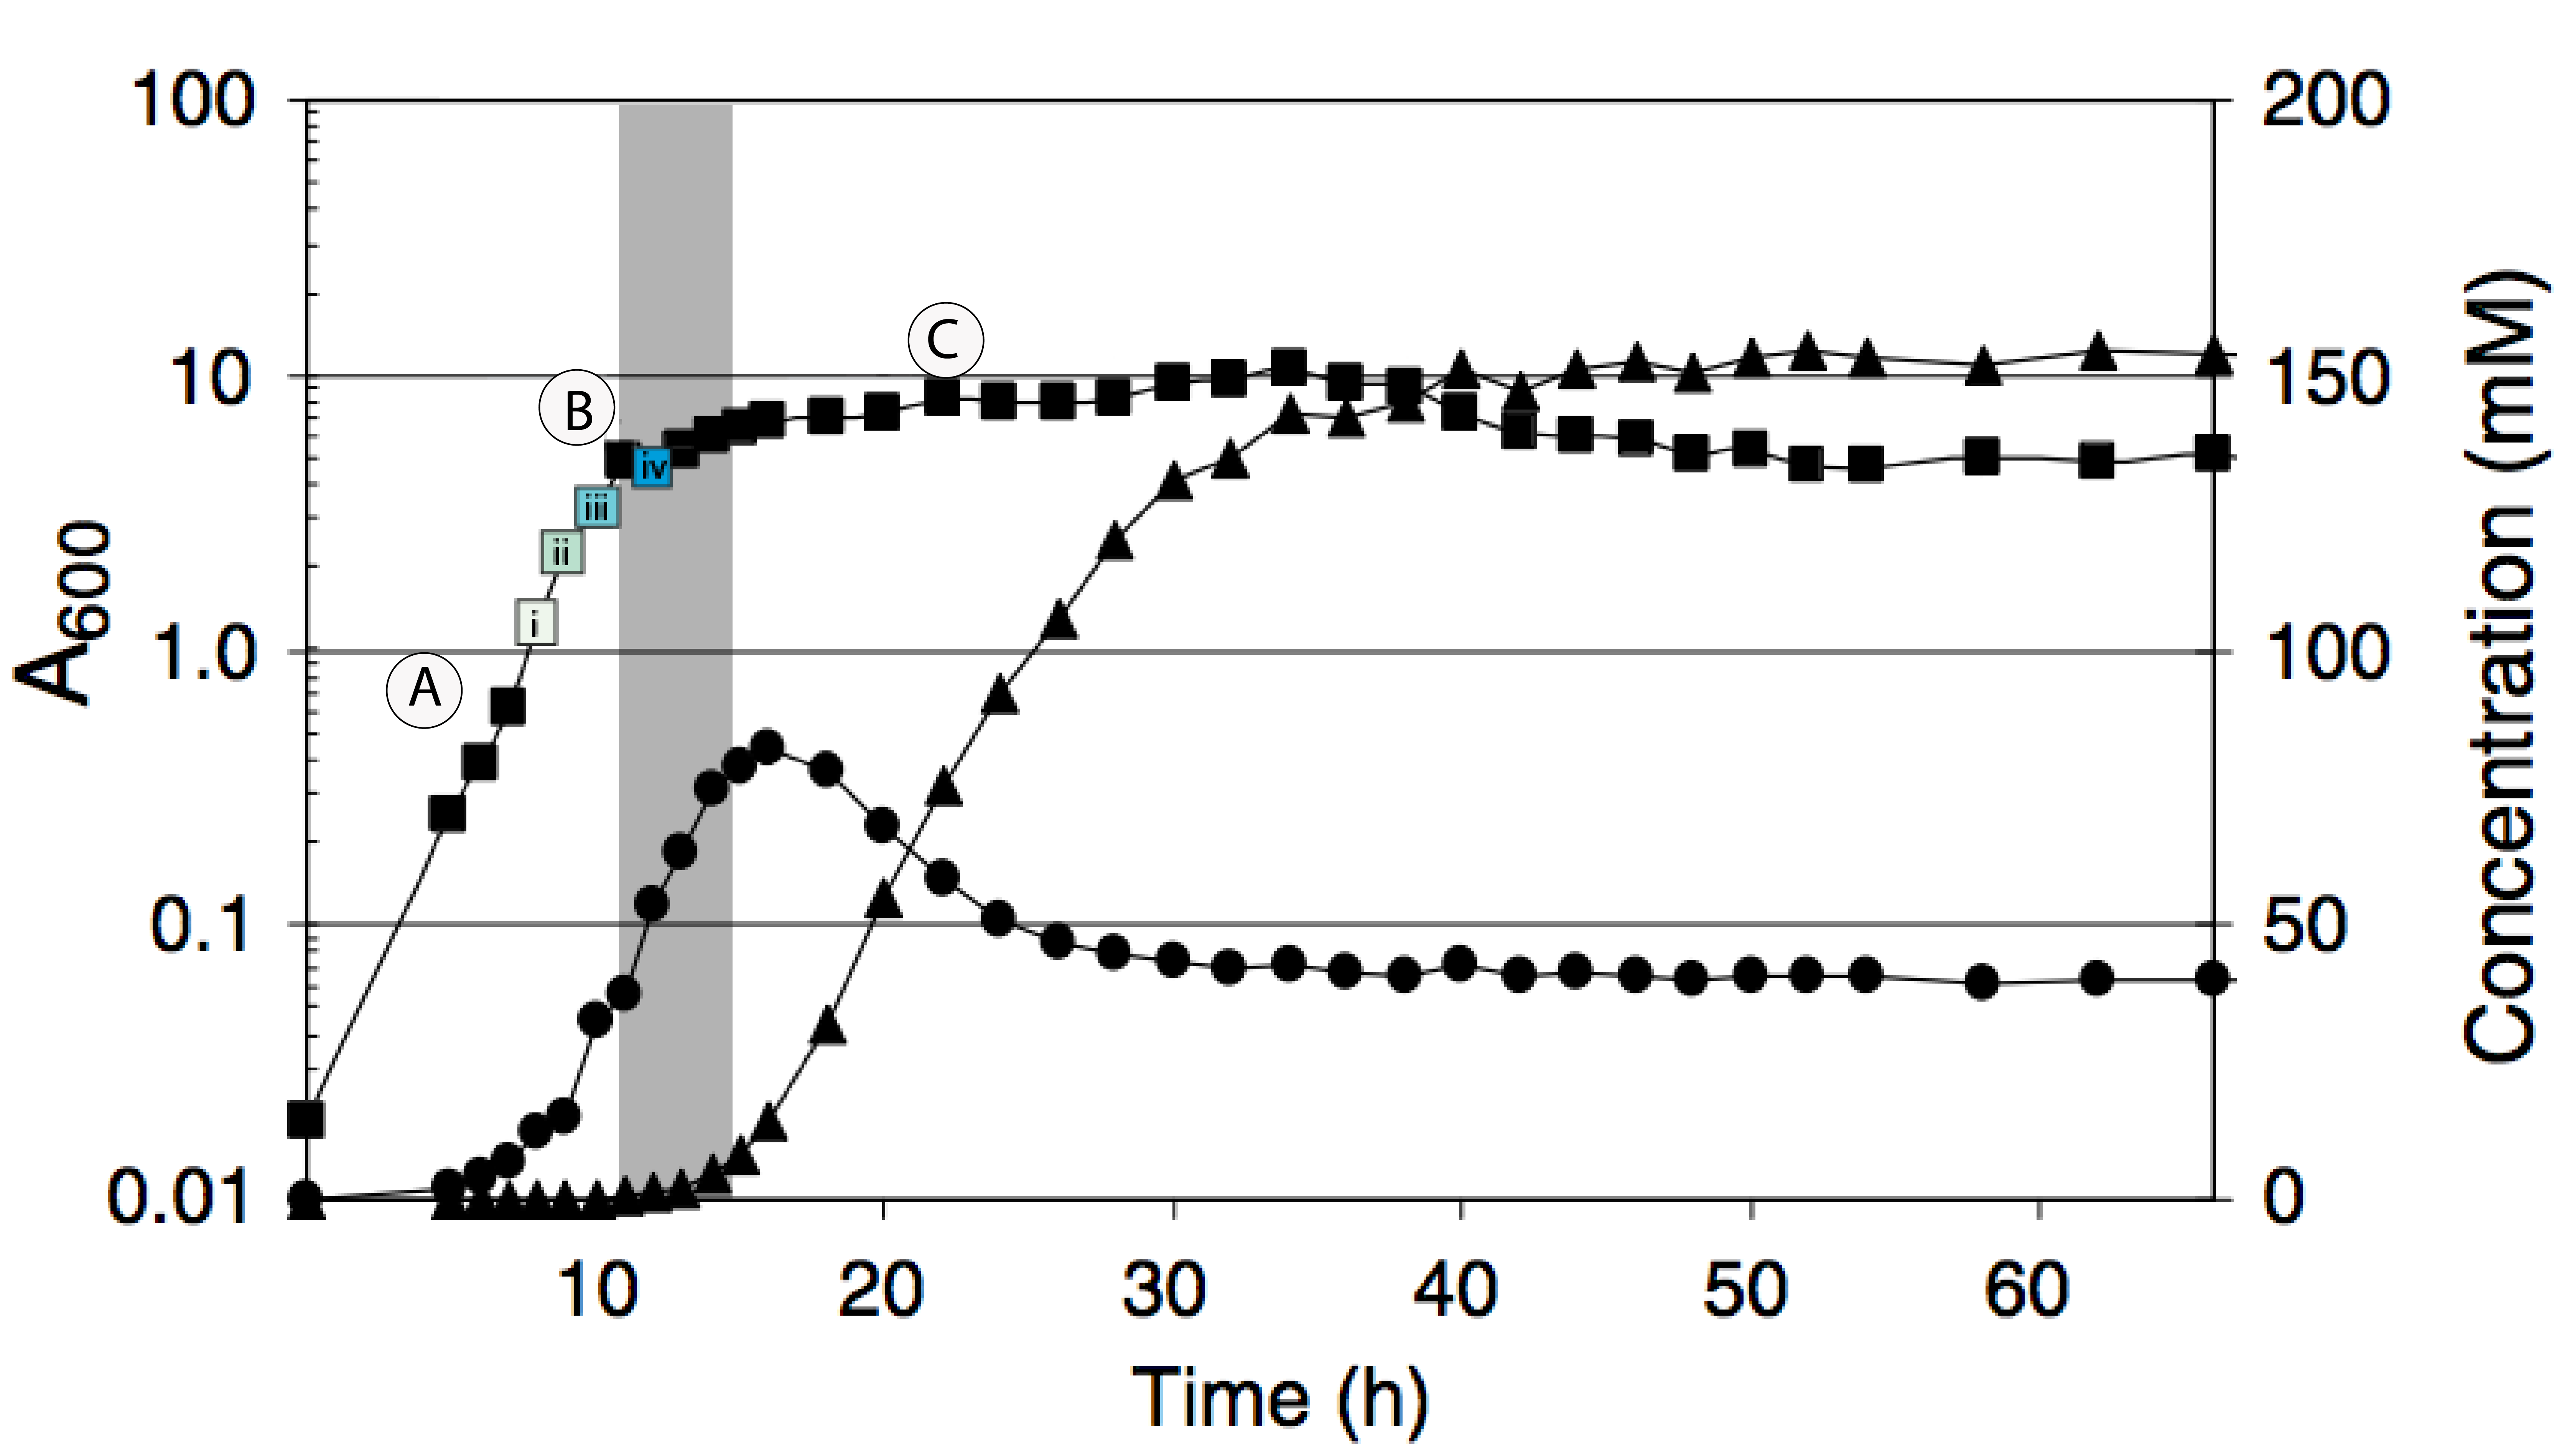
\includegraphics[width=\textwidth,height=3in]{images/Sequencing/Supplemental/Growth_curve.png}
\caption{\textit{C. acetobutylicum} Growth Curve}
\label{fig:1}
Populations of \textit{C. acetobutylicum} grow through the exponential phase ( A) A_{600} of 1.0), producing carboxylic acids, including butyric acid, during the transition phase (B). Then, the acids are reassimilated and reduced into solvents (C). These stressors were assayed in this experiment, in addition to time points 15(1.), 75(2.), 150(3.), and 270 minutes (4.) after synchronization at A_{600} of 1.0.
\end{figure}

RNA purity and integrity effect data quality. DNA contamination could effect the level of background signal. Small molecule, protein, or divalent cation contamination could degrade RNA or alter the effectiveness of the enzymatic reactions used in the preparation. RNA degradation effects the ultimate complexity of the library. To ensure RNA purity, after each step of RNA manipulation, the RNA was washed twice with 70\% alcohol, precipitated, and analyzed via spectrophotometry and the Agilent BioAnalyzer platform (\ref{methods:RNA_prep}). Ratios of absorbance ($\sfrac{\SI{260}{\nano\meter}}{\SI{280}{\nano\meter}}$, $\sfrac{\SI{260}{\nano\meter}}{\SI{230}{\nano\meter}}$) are frequently used to describe the purity of nucleic acid samples, due to purine/pyrimidine absorbance maxima at \SI{260}{\nano\meter}. Ratios of 2.0 indicate pure RNA, optimal for RNA-seq.

\begin{figure}
\hbox to \textwidth{\hfill
\rotatebox{90}{%
\begin{minipage}{\textheight}
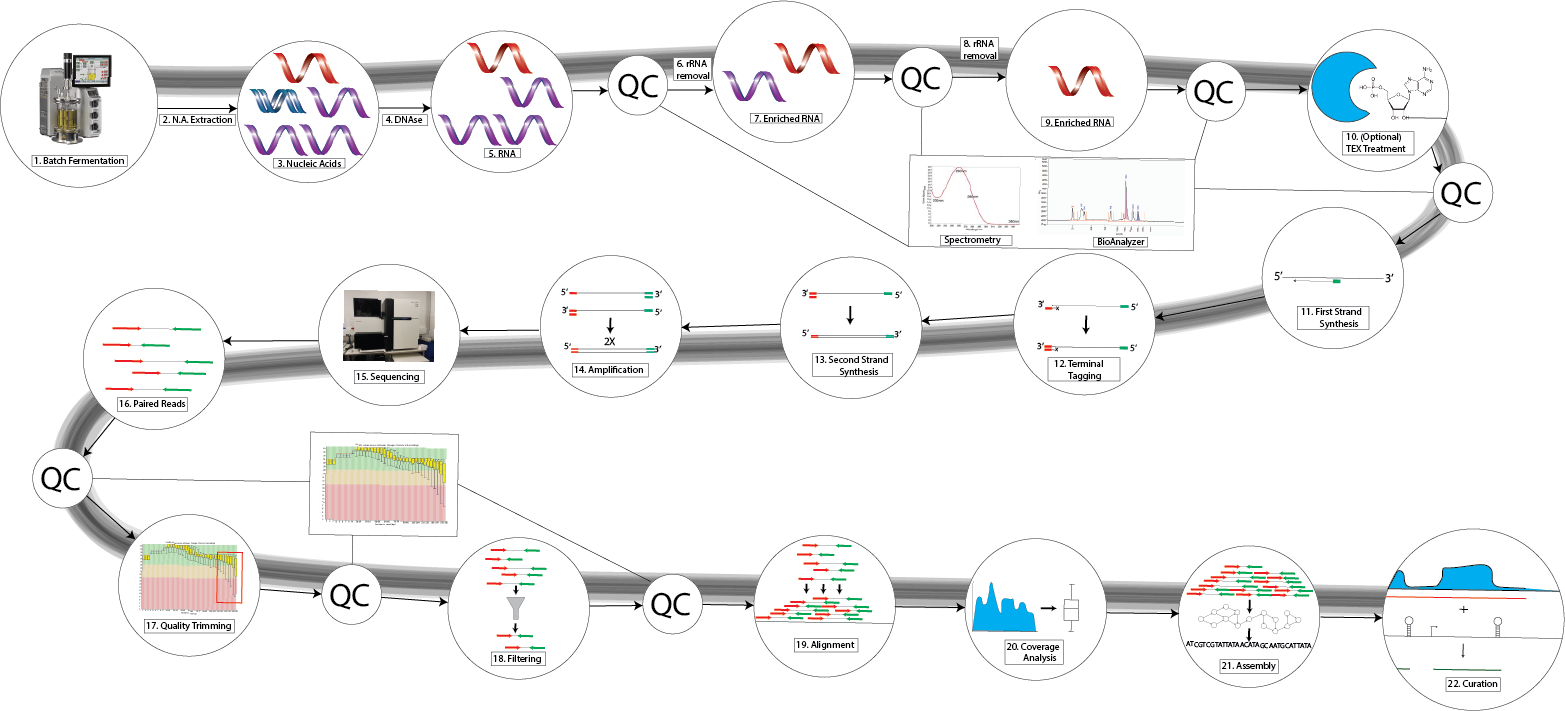
\includegraphics[width=\textheight,height=5in]{images/Sequencing/Supplemental/Workflow.png}
\caption{Laboratory Workflow}\label{fig:2}
The laboratory workflow consisted of mRNA enrichment steps and quality control analyses to ensure RNA quality. Ligation-free library preparation resulted in paired-end Illumina reads for preprocessing, alignment, analysis, and assembly.
\end{minipage}}\hfill}
\end{figure}

RNA integrity is commonly analyzed by interpreting ribosomal RNA bands. Specifically, a small peak width of the rRNA electrophoretic bands with little background signal indicates that the RNA high quality (e.g. RNA Integrity Number). A representative electropherogram is shown in \ref{fig:3}. The results clearly indicated high quality RNA with sharp, thin peaks for the 16S and 23S rRNA bands. With intact RNA, clear pellets, and clean spectrophotometric ratios, the RNA were then used for library preparation and sequencing. 

\begin{figure}
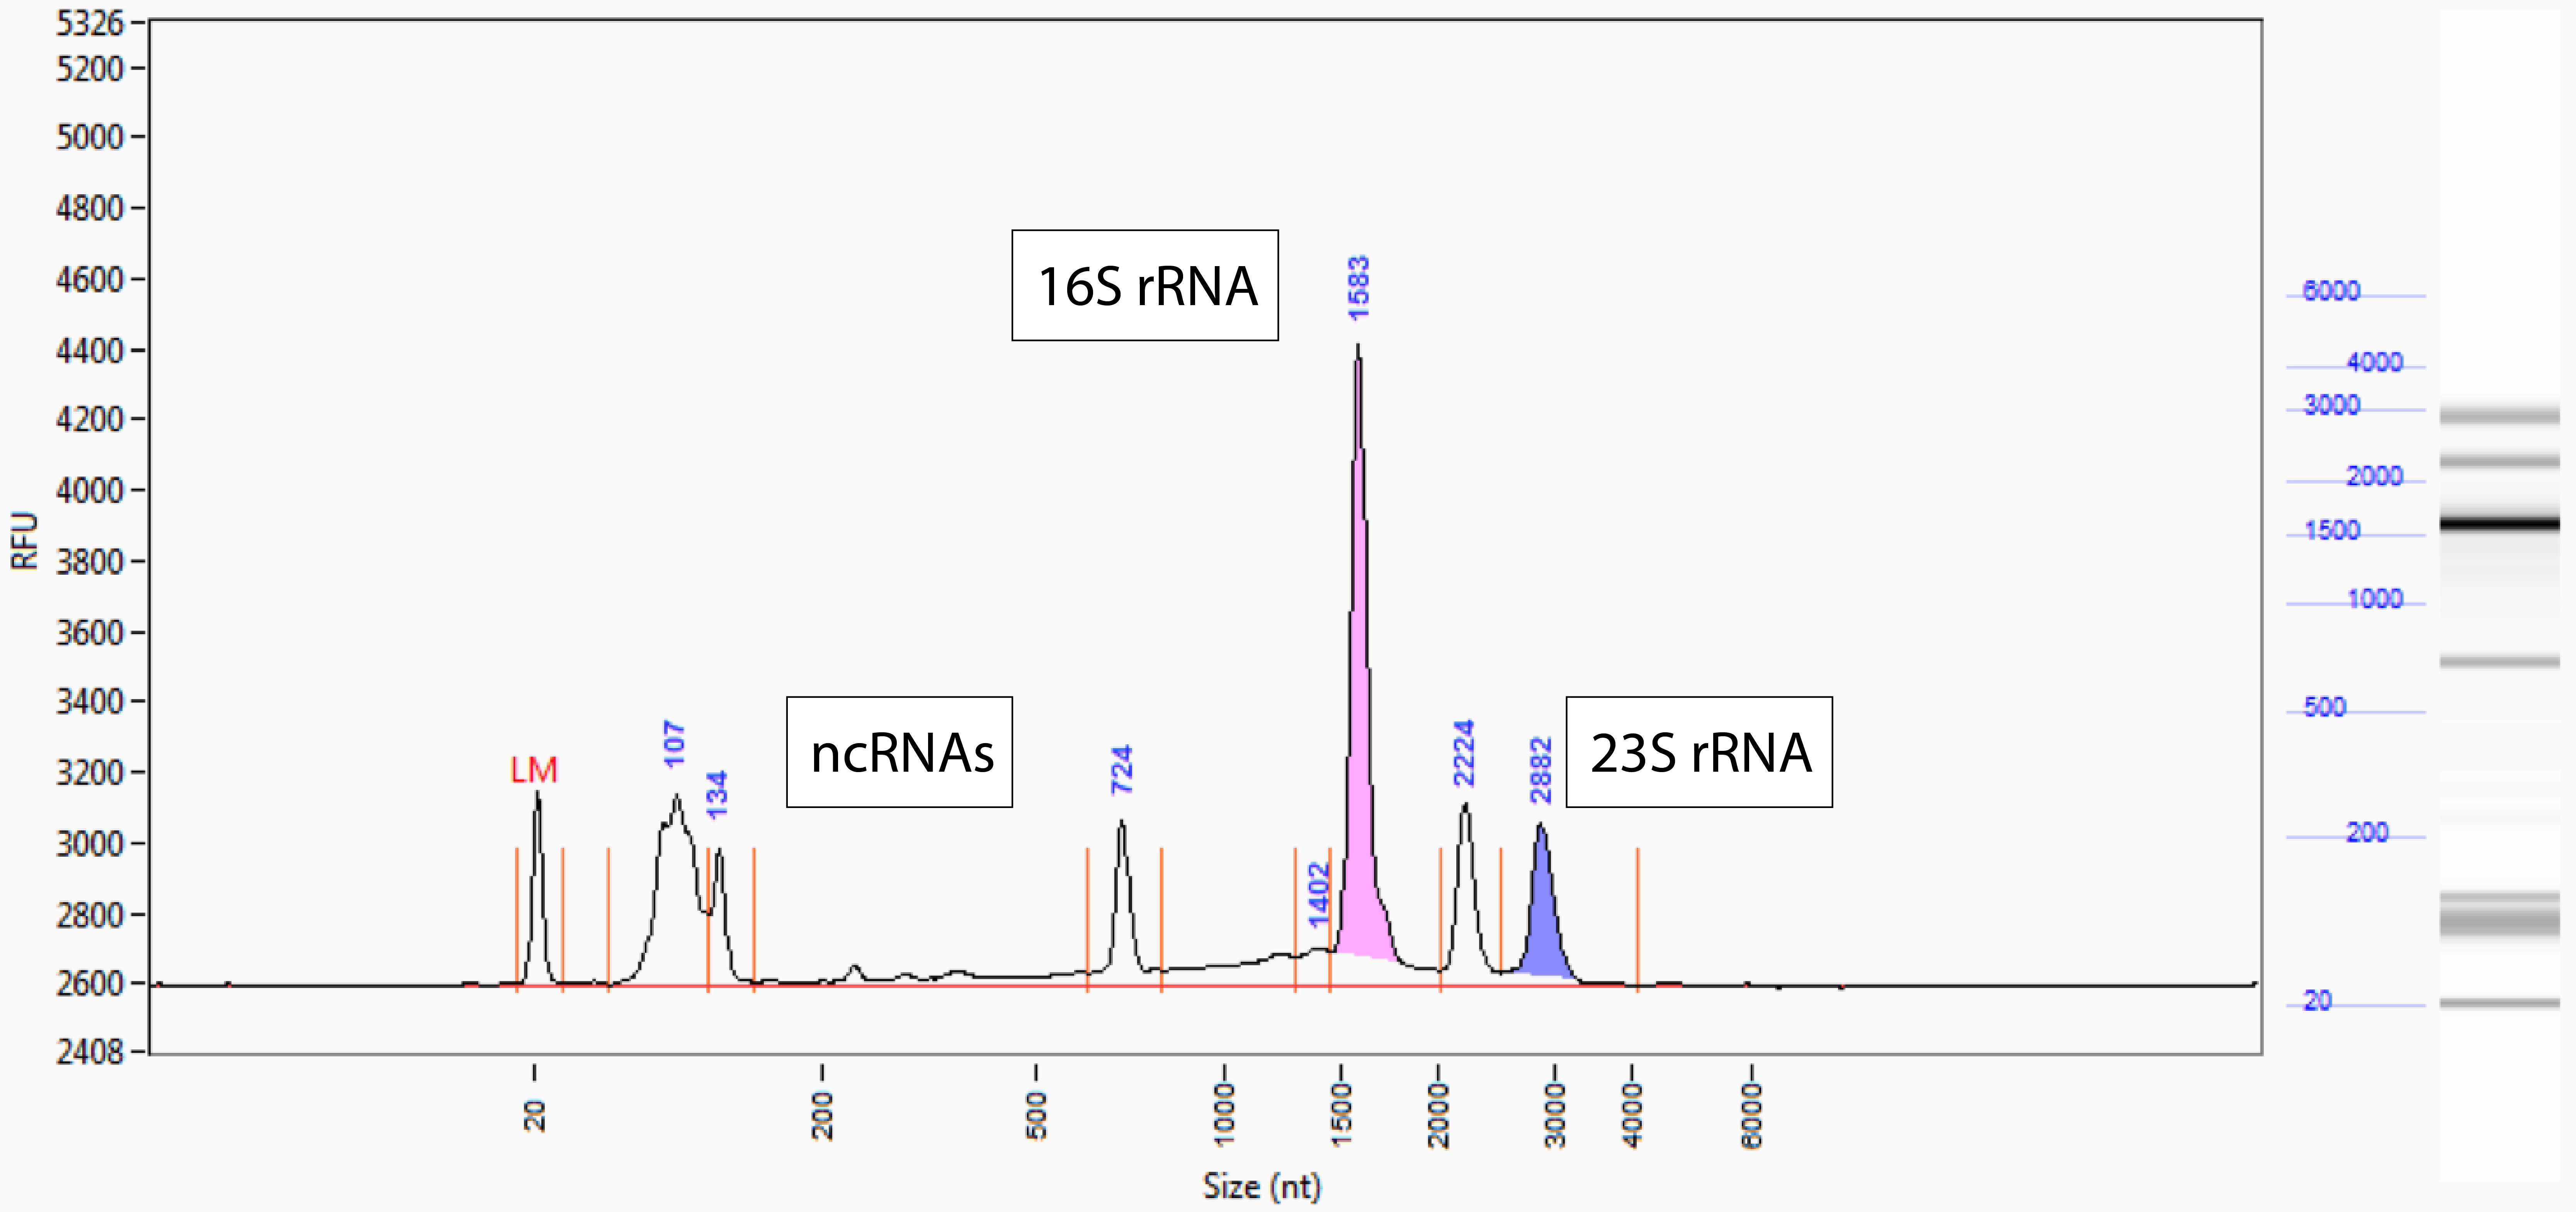
\includegraphics[width=\textwidth,height=3in]{images/Sequencing/Supplemental/RNA-integrity.png}
\caption{RNA Quality}\label{fig:3}
\end{figure}

\section{Data Processing, Alignment, and Coverage Analysis}
The libraries were sequenced paired-end over 6 lanes of an Illumina HiSeq 2500, producing 1.5 billion 75bp reads, averaging 25 million clusters/pairs per library. The reads were then processed through a customized bioinformatic workflow (\ref{methods:data_proc_aln}), first trimming low-quality bases, then filtering ribosomal RNA reads, and finally aligning to the genome (\ref{fig:2}). On average, 97\% of the useful, non-ribosomal reads were aligned to the \textit{C. acetobutylicum} genome. Of these, 7.75M(83\%) were properly paired, that is, both mates of each pair were in the correct orientation. In total, 458,814,860 perfectly paired reads were produced and then used for subsequent analysis. 

\newgeometry{left=2cm,right=2cm,top=1cm,bottom=1.5cm}
% Reads per library table
\begin{table}
%\hbox to \textwidth{\hfill
\rotatebox{90}{%
\begin{minipage}{\textheight}
\caption[Read Summary]{Read Summary}
\begin{tabular}{|l| *{12}{c|} }\hline%
ID & Stress & Time & Rep. & Barcode & Lane & Total & rRNA & non-rRNA & Mapped & Chrom. & pSol1 & Proper-pairs\\\hline\hline
\csvreader[late after line=\\\hline]%
{tables/Reads_Summary.csv}
{id=\id, stress=\stress,time=\time,replicate=\replicate,barcode=\barcode,lanes=\lanes,total=\total,rRNA=\rRNA,nonrRNA=\nonrRNA,mapped=\mapped,chromosomal=\chromosomal,pSol1=\pSol1,properlypaired=\properlypaired}{\id & \stress & \time & \replicate & \barcode & \lanes & \total & \rRNA & \nonrRNA & \mapped & \chromosomal & \pSol1 & \properlypaired}
%{id=\id, stress=\stress, time=\time, replicate=\replicate, barcode=\barcode, lanes=\lanes, total=\total, rrna=\rRNA, nonrrna=\nonrRNA, mapped=\mapped, chromosomal=\chromosomal, psol1=\pSol1, properlypaired=\properlypaired}%
%{\id & \stress & \time & \replicate & \barcode & \lanes & \total & \rRNA & \nonrRNA & \mapped & \chromosomal & \pSol1 & \properlypaired}%
\end{tabular}
\end{minipage}}
%\hfill}
\end{table}
\restoregeometry
%\csvautotabular{tables/Reads_summary.csv}



%\begin{figure}
%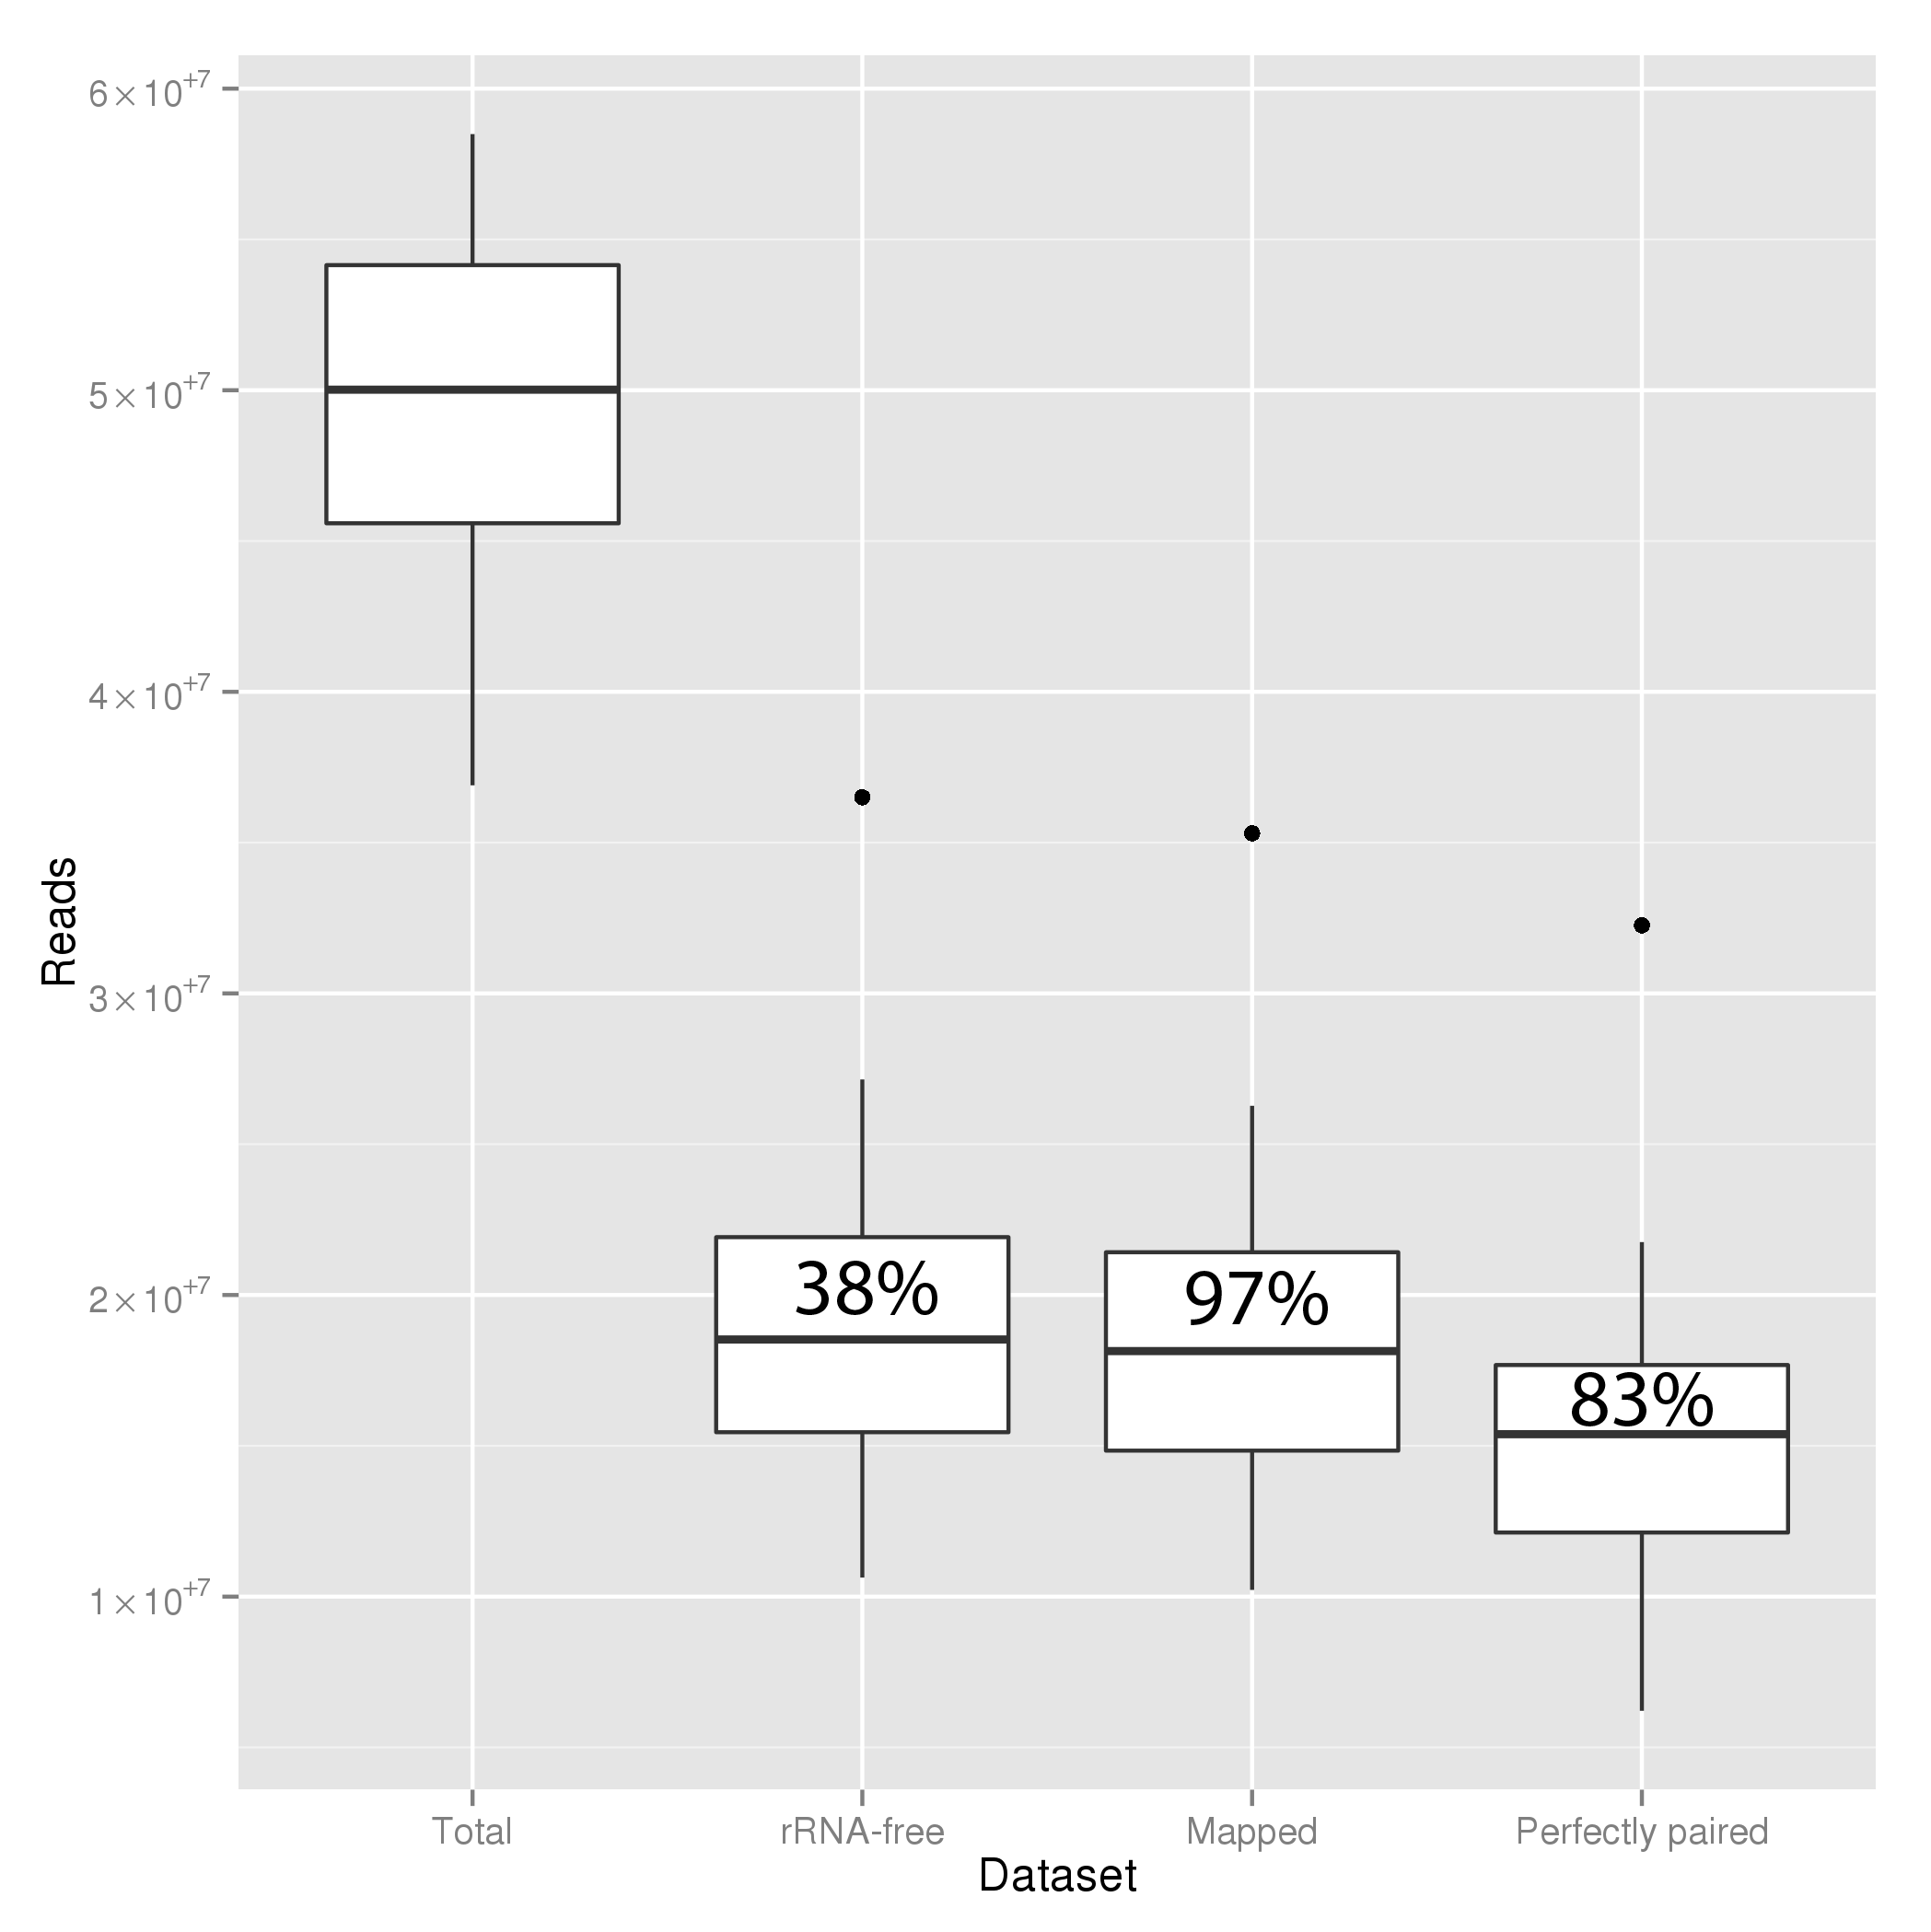
\includegraphics[width=\textwidth,height=3in]{images/Sequencing/Alignment_brief.png}
%\caption{Sequence Read Processing and Alignment}\label{fig:4}
%An average of 50 million reads (25M clusters/pairs) was produced for each of the 30 libraries. Ribosomal RNA reads were then filtered and the remaining reads were then aligned to the genome. Of these, 83\% were properly paired reads, ideal for transcriptome assembly.
%\end{figure}

After read alignment, it was desirable to determine the per base sequencing coverage across the genome.  The Encyclopedia of DNA Elements (ENCODE) project has released best practices guidelines for RNA-seq projects (Source??). Empirically, it seems that a coverage of 100-200M 100bp paired-end reads is sufficient to detect low abundance transcripts in the 60-140 megabases(Mb) hg19 human transcriptome. This sums to 20-40Gb of sequencing, 120-660x through a back of the envelope calculation, with a very conservative estimate of the size of the human transcriptome. In the case of \textit{C. acetobutylicum}, the upper boundary on the transcriptome is 8.2Mb, with a realistic estimate between 4-6Mb. With just the properly paired reads, 68.7Gb were sequenced for a much smaller transcriptome, approximately 11-17k times the length of the transcriptome. This estimate suggests that cumulatively, this study achieves comparable or superior depth than recommended by these guidelines. 

However, this estimate poorly represents the actual distribution of coverage per base throughout the transcriptome. A median of > 10x coverage per base and per strand was observed for each of the 30 libraries (ref{fig:5a}). Cumulatively, the median per base coverage is 156x throughout the genome(ref{fig:5b}). It is likely that in truly transcribed regions, the coverage is greater. Rather, some of the coverage described by this distribution is likely due to background signals from the RNA-seq technique. Background signal is indeed a pressing concern for RNA-seq (ENCODE source), potentiall from residual DNA escaping the RNA purification, DNAse digestion, and spectrophotometric analyses of the laboratory workflow. 


%\begin{figure}
%{\includegraphics[width=\textwidth,height=3in]{images/Sequencing/Example_coveragepng}
%\subcaption{Representative Genome Coverage Distribution}\label{fig:5a}}
%{\includegraphics[width=\textwidth,height=3in]{images/Sequencing/Cumulative coverage.png}
%\subcaption{Cumulative Genome Coverage Distribution}\label{fig:5b}}
%\caption{Coverage Boxplots}
%\subref{fig:5a}) Initial co
%\end{figure}



% This is the section of the results focused on the assembly


\chapter{Transcriptome Assembly}

\section{Assembly Quality}

\subsection{Quality Statistics}


A primary motivation for the assembly and subsequent annotation has been the amount of data(reads) that are accounted for in the existing/reference annotation. An average of 1.7 million reads per sample are accounted for in these regions, out of an average of 10[M]illion rRNA-free reads.  Only 17\% of the usable, quality data are accounted for by the coding sequences of the reference annotation. However, 10M reads exceeds the typical sample depth for comparable efforts of transcript boundary identification. For these reasons, transcriptome assembly is necessary for transcript boundary identification.

4177 transcripts (7.18Mb from a 8.3Mb genome) were assembled, after removing duplicates. Each of these transcripts aligned to one location in the genome with \textgreater 98\% identity and less than 30bp of gaps. Of these, 1057 transcripts spanning 4.56Mb (25\% by the number of assembled transcripts;  63.5\% by assembled basepairs) contain 3287(86\%) reference ORF or one of 60 novel CDSes.  The remaining 3120 (75\% by number, 36.5\% by basepairs) of transcripts are novel (Fig. 1. Orange) and their lengths range from 200-32.7kb. The reference-ORF containing transcripts will be referred throughout as the ``standard'' set of transcripts and most of the investigation below describes this group.

The standard set of transcripts were larger on average by approximately an order of magnitude.

\begin{figure}
\begin{center}
\begin{minipage}[b]{2.25in}
\resizebox{2.25in}{2.5in}{
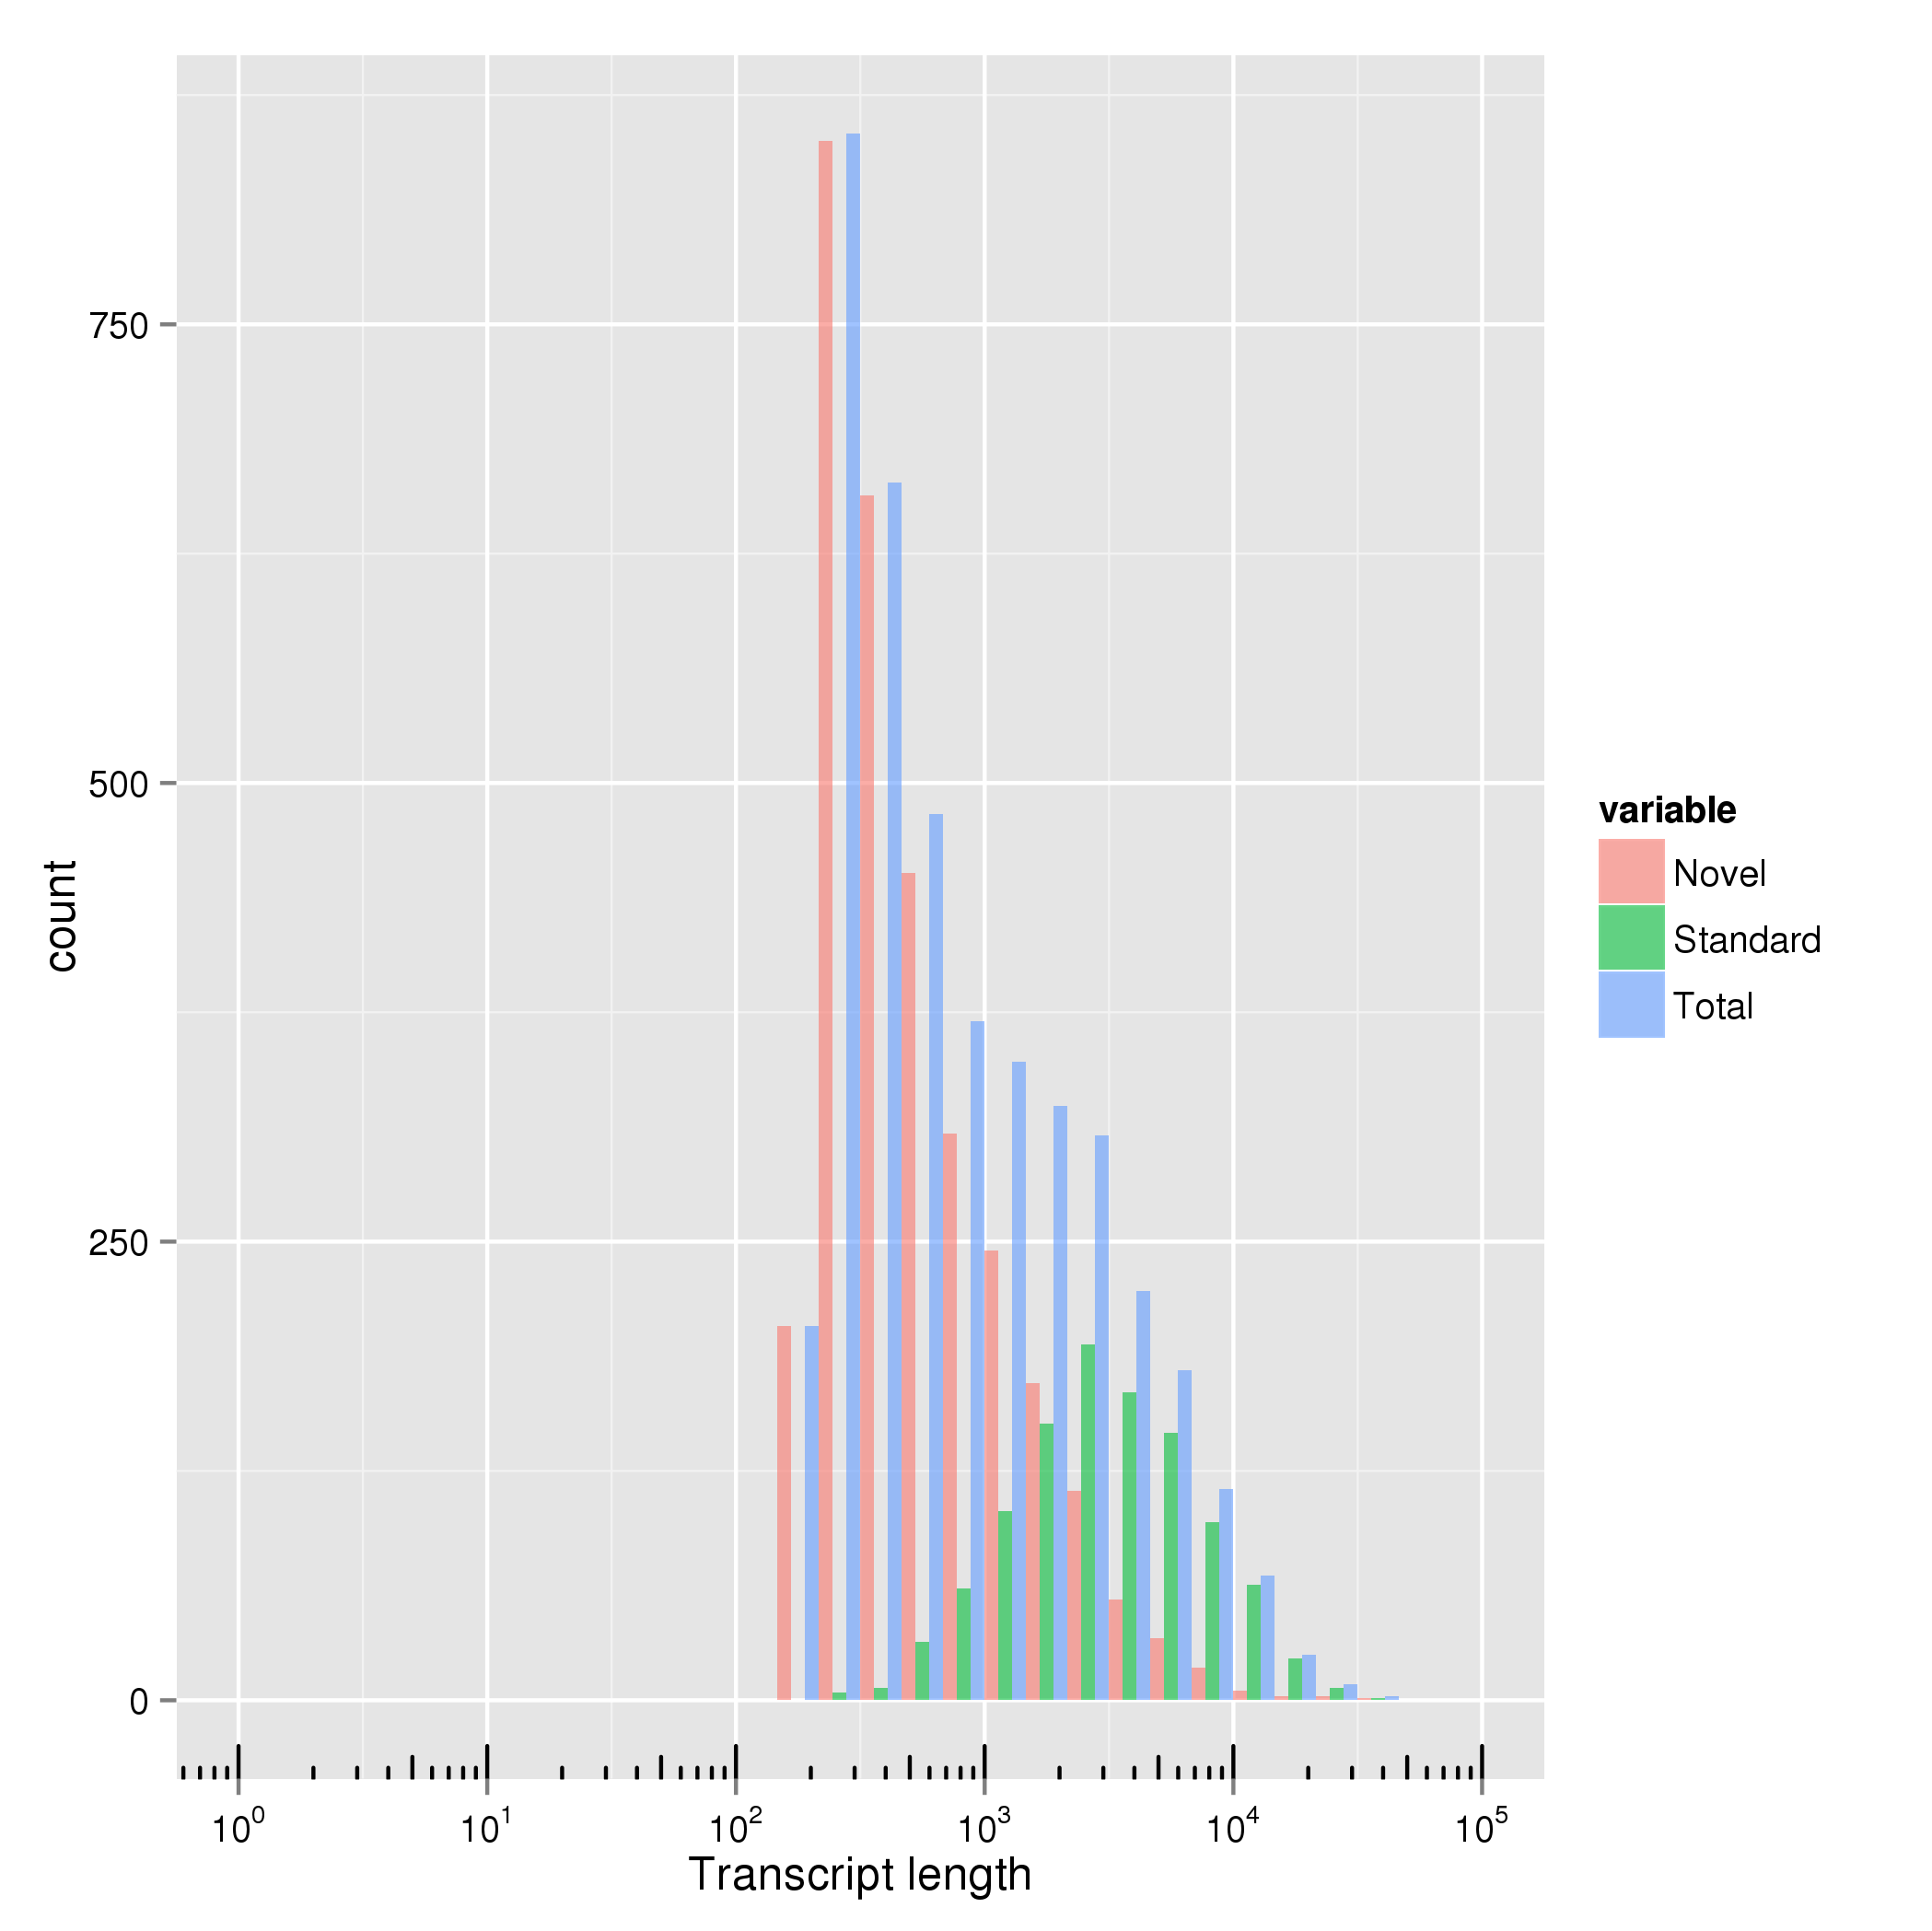
\includegraphics{images/Assembly/Summary/ftranscript_length.png}

}

\end{minipage}

\begin{minipage}[b]{2.25in}
\resizebox{2.25in}{2.5in}{
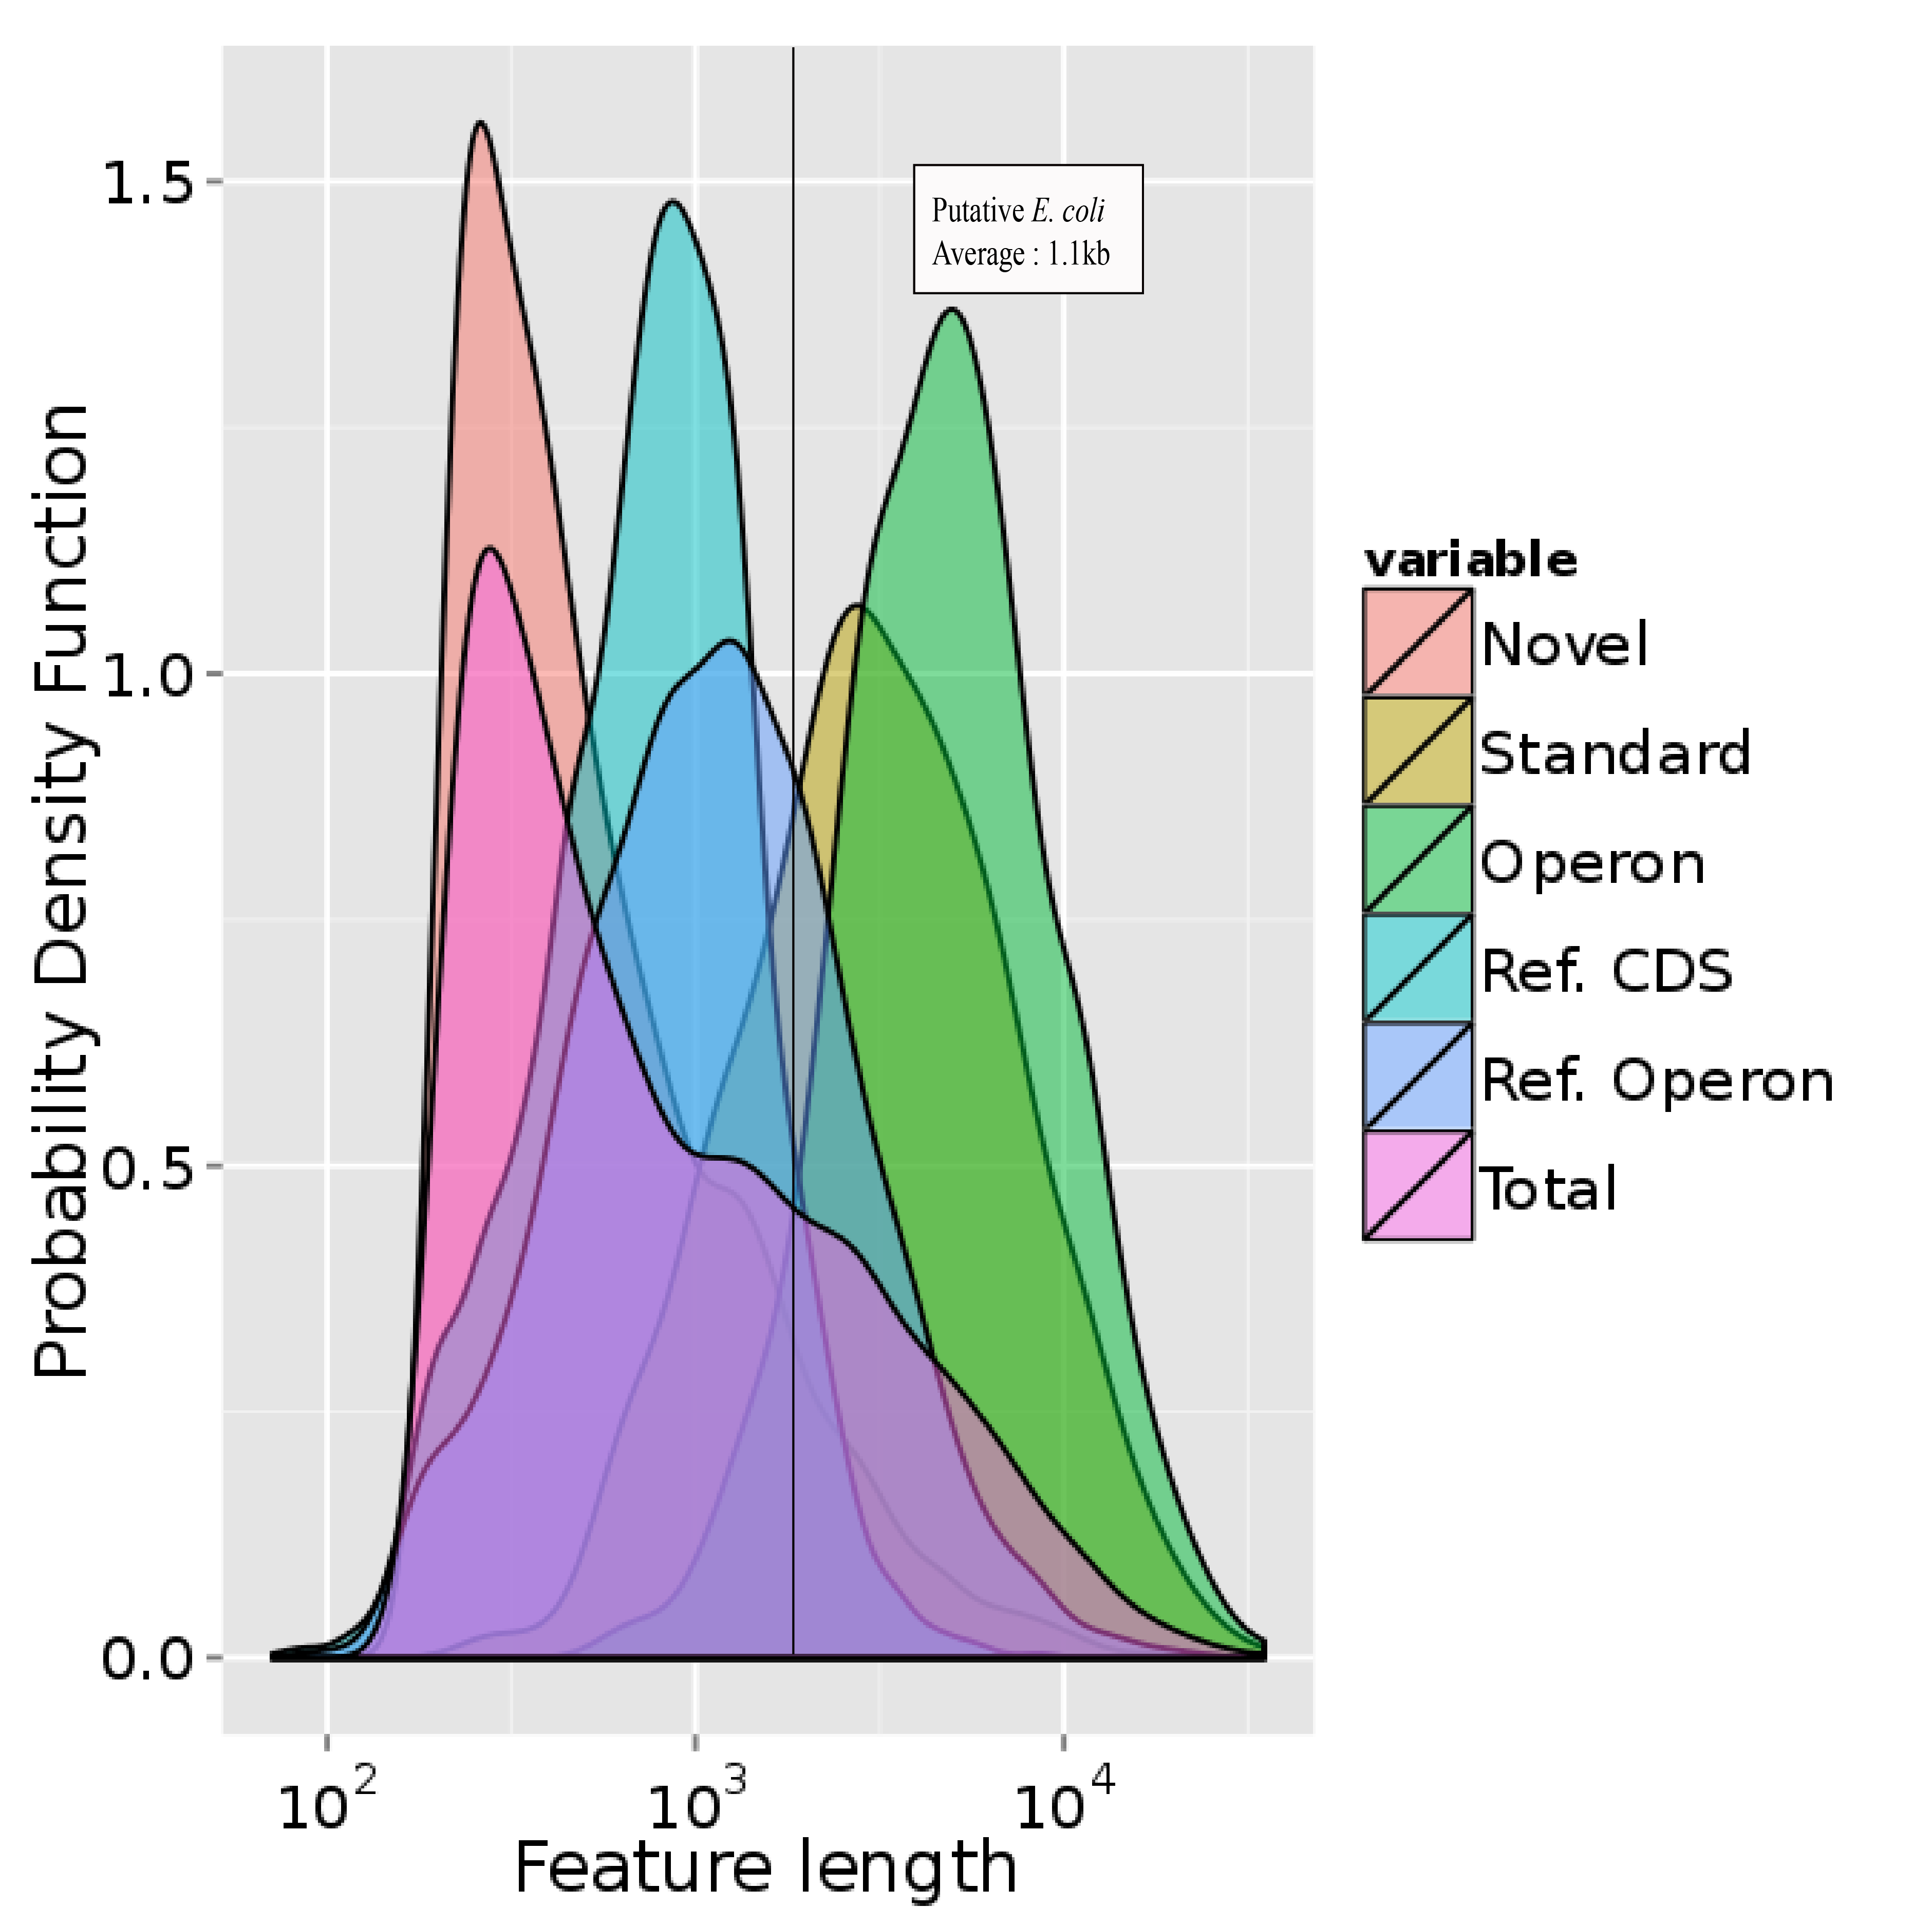
\includegraphics{images/Assembly/Summary/ffeature_length_1.png}
}

\end{minipage}
\end{center}

\caption{Transcript and Feature Length Distributions}
\end{figure}




\subsection{Example Transcripts}


To assess the data/assembly quality further, I used canonical transcripts of \textit{C. acetobutylicum}, to understand the agreement of the coverage, the assembly, and the existing annotation. Six issues, listed below, were considered for each example to better understand the quality of the assembly and the degree of curation required. 

\begin{enumerate}
\item Is the transcript large enough to include the known ORFs and RBSes?
\item Does the assembled transcript's TSS agree with promoter motifs?
\item Does it agree with published transcription start sites?
\item Does the assembled transcript's size agree with published Northern blots?
\item Does the assembly represent the coverage and if not, which of these two best represents the biological knowledge of this region?
\item Does the assembled region require curation (e.g. fused, extended, or truncated transcripts)?
\end{enumerate}

Agreement between the data and the literature would support the efficacy of this technique. Its effectiveness is particulary important in cases where no previous experimental data exists. These results could be very useful to future studies if only minimal remediation or curation is required. The first example that I examine is the Sol locus.

\subsubsection{Sol Locus}

The Sol locus is a 7kb region on the pSol1 megaplasmid surrounding the Sol operon(4.3kb, basepairs 175,564-179,841). This region is responsible for the production of several solvents\cite{62,63}. This region encodes several enzymes including a tri-functional NAD(H\textsuperscript{+})-dependent alcohol/aldehyde dehydrogenase (AdhE)\cite{62}, two subunits of coenzyme-A transferases (ctfA/B)\cite{66}, and an acetoacetate decarboxylase (Adc)\cite{64,65,66}. The region is also home to a protein SolR, which includes a helix-turn-helix motif and is thought to regulate solventogenesis\cite{67}. These genes are vital for carboxylic acid reuptake and conversion into alcohols, a vital part of this organism's metabolism and the solventogenesis process.

%          SOL LOCUS Fig 1.
\begin{figure}
\small
{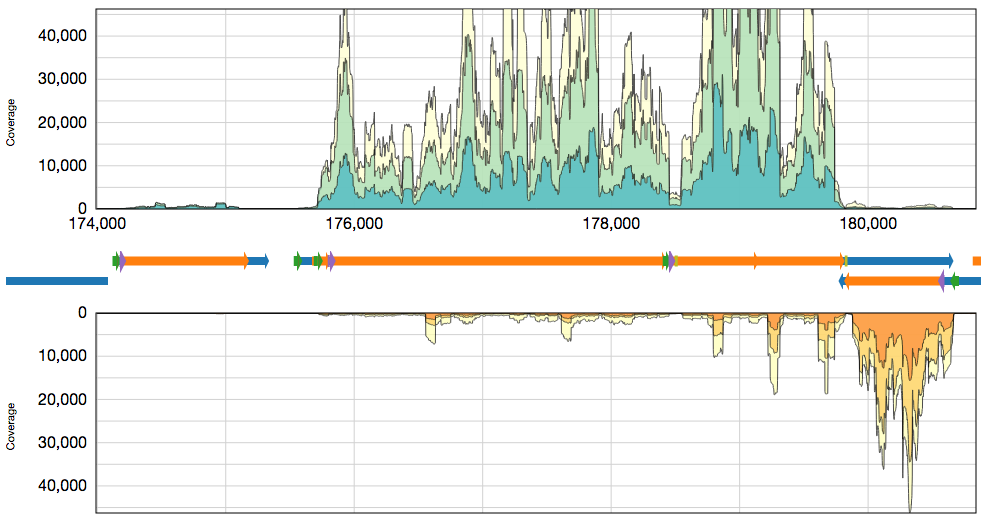
\includegraphics[width=\textwidth,height=2.5in]{images/Assembly/Examples/Sol/Sol-locus.png}
\subcaption{Sol locus}\label{fig:1a}}
% \label{fig:1}
\caption{Sol Locus Overview} This operon (\subref{fig:1a}) upper track) consists of OrfL, alcohol dehydrogenase (AdhE), and Co-A transferases A and B (ctfA,ctfB). SolR (far left) and acetoacetate decarboxylase (ADC; \subref{fig:1a} lower track, right) are also shown. Coverage for the Watson and Crick strands (top and bottom tracks) are visualized with an annotation track (center). Tracks show cumulative coverage for unstressed (yellow), butanol (light green/ light orange), and butyrate (green/orange) stressed samples over all time points. Transcripts (blue), ORFs (orange), RBSes (purple), inverted repeats (yellow), promoters (green), and TSSes (red) are represented as arrows and bars.
\end{figure}

\paragraph{Acetoacetate Decarboxylase Transcript}
In the early 1990s, several articles were published about the Sol locus including the cloning and sequencing of Adc and the Sol locus\cite{62,63,64,65,66}. An early study of the Sol operon probed the Adc locus, reporting two transcript sizes of 670 and 865 with Northern blot\cite{65}. The authors also reported the major transcription start site of Adc at base 180671 of the pSol1 plasmid. To examine the quality of our data and raw assembly, we examined this locus to observe the transcript size and locate the transcription start site in our data. In \ref{fig:2a} we see the transcription start site reported by Durre(red) located very near a sustained increase in sequencing coverage just downstream of a canonical promoter motif. This pattern of coverage (cumulatively \textgreater 10,000x) is sustained until a bidirectional Rho-independent terminator (\ref{fig:2b}). In this instance, the precise transcription start site was not estimated precisely by the uncurated assembly. The reported transcript continues for several hundred basepairs upstream of the Adc TSS, despite the decrease in coverage. This artifact is most likely due to sufficient k-mer complexity in the reads mapping upstream of the TSS for the Adc transcript to be fused to signal from genes upstream. Correcting for this error (\ref{fig:2c}), the full transcript size is 857. It was claimed that the 670bp product is most likely a specific degradation product or the result of a secondary transcriptional start site\cite{65}. To investigate this, a transcript of this size would correspond to a transcriptional start site at approximately base 180,484. Unfortunately, none of the promoter motifs in the region could explain a transcript of this size in vegetative cells. After curation based on the coverage pattern, promoter and terminator motifs in this region, the transcription start site and transcript size for Adc accurately match previous results. 

\begin{figure}
\small
{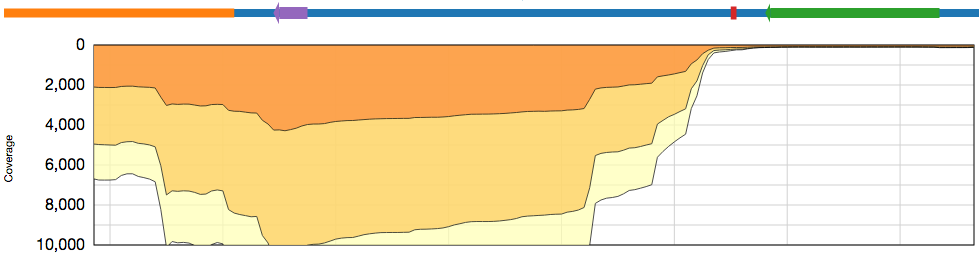
\includegraphics[width=\textwidth,height=1.5in]{images/Assembly/Examples/Sol/Sol-Adc-TSS.png}
\subcaption{Adc transcription initiation region on the Crick strand.}\label{fig:2a}}
{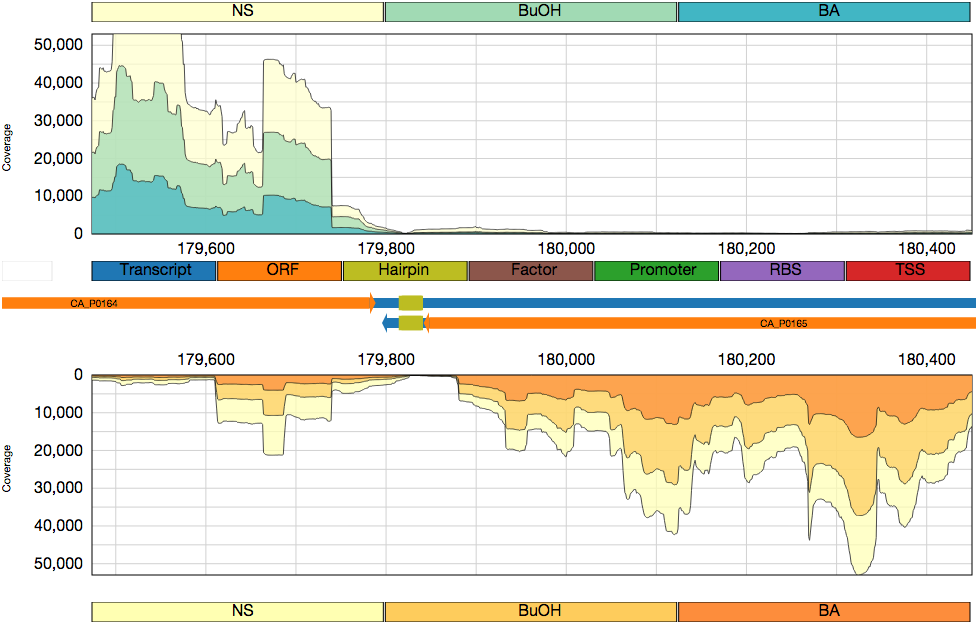
\includegraphics[width=\textwidth,height=2.5in]{images/Assembly/Examples/Sol/Sol-bifunctional-terminator.png}
\subcaption{Bifunctional Rho-independent terminator for Sol operon (upper track, left), Adc}\label{fig:2b}}
{\includegraphics[width=\textwidth,height=1.5in]{images/Assembly/Examples/Sol/Sol-Adc-curated.png}
\subcaption{Curated Adc locus}\label{fig:2c}}
\caption{Adc locus}
\subref{fig:2a}) Transcription initiation region for Adc. While the coverage clearly shows the appropriate increase, the transcription start site has been fused to residual coverage upstream of the true TSS. \subref{fig:2b}) A bifunctional terminator is responsible for transcriptional termination of both Adc and the Sol operon. \subref{fig:2c}) With minor curation, the region matches previous results faithfully.
\label{fig2}
\end{figure}


\paragraph{Sol Operon}
These studies additionally describe the Sol operon. In \cite{65}, Durre et al. examined the Sol operon using a probe specific for ctfB and reported a transcript size of 4.1kb. Unfortunately, no blots were included as figures in this work. In \cite{63} AdhE-based probes revealed a nearly identical transcript size of 4.1-4.2kb. Interestingly, the Sol operon has both proximal and distal transcription start sites at 175,726 and 175,564, respectively\cite{62,63}. Ribosome binding sites have been identified upstream of AdhE, CtfA, and CtfB\cite{63}. The expression level of the Sol operon is substantial, also upwards of 10,000x coverage cumulatively. The distal transcription start site is matched perfectly (\ref{fig:3a}), demonstrating the precision of the assembly technique in the absence of background or residual signal. An increase in coverage is observed immediately following the proximal promoter (\ref{fig:3a}) in close agreement with the previous determinations\cite{62,63}. However, the transcription stop site was not precisely determined by the assembly, owing in part to basal antisense signal from the Adc gene (\ref{fig:2b}). After adjustment, the transcript sizes are 4,115 and 4,277, respectively, in close agreement with the reported transcript sizes\cite{63,65}.

\begin{figure}
\small
{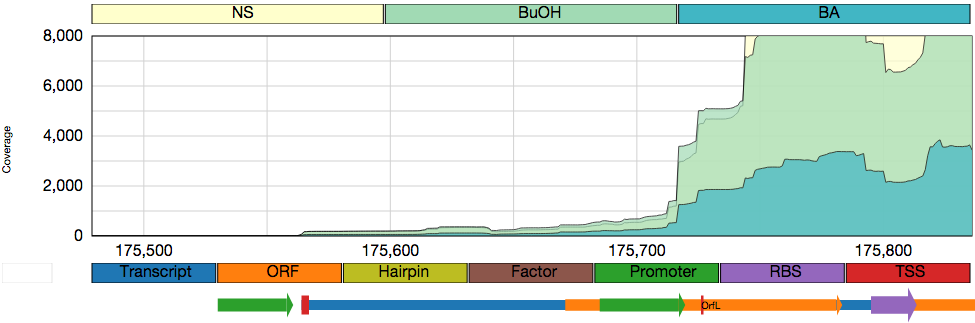
\includegraphics[width=\textwidth,height=1.5in]{images/Assembly/Examples/Sol/Sol-TSS.png}
\subcaption{Sol operon transcription initiation region. The distal (left) and proximal (right) transcription start sites (red) are shown for AdhE (far right, orange).}\label{fig:3a}}
{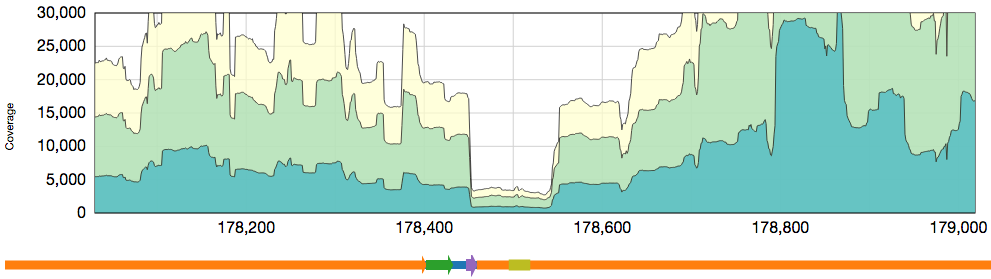
\includegraphics[width=\textwidth,height=1.5in]{images/Assembly/Examples/Sol/Sol-AdhE-terminator.png}
\subcaption{Putative AdhE (left) terminator, CtfA (right) promoter}\label{fig:3b}}
\caption{Sol Operon}
\subref{fig:3a}) Sol operon (OrfL, center; AdhE right) transcription start sites. The coverage and assembly data have strong agreement with previously described proximal and distal promoters and transcription start sites. \subref{fig:3b}) Low coverage in the Sol operon. A terminator may be partially responsible for a sustained low coverage level in the Sol operon. Additionally, a promoter motif was located upstream of the CtfA RBS and the pattern of expression is consistent with these observations.
\end{figure}

\paragraph{Multiple Transcripts from Sol Operon}
While the results from this region agree as a whole, there is an interesting pattern in coverage in the Sol operon near the C-terminus of AdhE(\ref{fig:3b}. This 100bp region is expressed at a statistically lower level (K.S.-test, p < 0.05) than the rest of the Sol operon. Upon further examination of this region, we find a Rho-independent terminator with a \(\Delta\)G of -9.6 kcal/mol, which is not as strong as the -11.5 kcal/mol bifunctional terminator at the end of the Sol operon. The region is also near a Sigma-A promoter motif of TTCATA(13)TATAAT located upstream of the previously mentioned RBS. As mentioned above, no Northern blots figures were included in the only study, to the best of my knowledge, that uses ctfA or ctfB specific probes\cite{65}. Most studies of the Sol operon in \textit{C. acetobutylicum} use AdhE-specific probes or larger restriction digestion probes \cite{63,68,70}. One of these displays a Northern with a weak but distinct band for a ~2.6kb transcript under solventogenic conditions \cite{68}. If AdhE were transcribed both in the classical Sol operon and as a separate transcript, the length would be 2,716bp from the proximal transcription start site. This pattern of coverage is consistent across all replicates. This length of the pattern suggests this observation does not merely represent difficulty sequencing secondary structure in the Sol operon transcript. In addition to the full Sol operon transcript, additional transcripts from the AdhE and ctfA/B genes may be produced.


\paragraph{SolR Transcript}
The last transcript produced from the Sol locus considered here is that of the SolR gene. This gene produces two transcripts, one 1kb and the other 1.3kb\cite{63}. A later study revealed the role of SolR as a repressor for the Sol operon\cite{67}. This study also produced a single transcription start site at 174,154 on the pSol1 plasmid. As a result of examining this dataset, we see a perfect recapitulation of the transcription start site (\ref{fig:4a}). The transcript from the raw assembly is approximately 1.2kb, showing only residual coverage (cumulatively \textless 5x) after the first terminator. After curation (\ref{fig:4b}), the transcript size is 1,036bp. There was insufficient coverage in the conditions studied to strongly support the larger transcript and no alternative transcription start sites were apparent.


% Transcription start sites SolR
\begin{figure}
{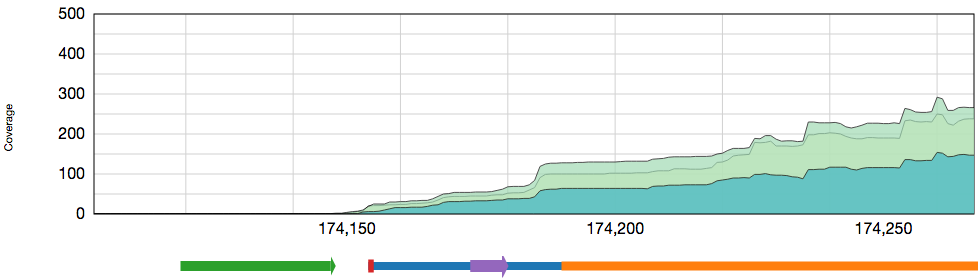
\includegraphics[width=\textwidth,height=1.5in]{images/Assembly/Examples/Sol/Sol-SolR-TSS.png}
\subcaption{SolR transcription initiation region}\label{fig:4a}}
{\includegraphics[width=\textwidth,height=1.5in]{images/Assembly/Examples/Sol/Sol-SolR-curated.png}
\subcaption{Curated SolR Transcript}\label{fig:4b}}
%\label{fig:1.5}
\caption{SolR Locus}
\subref{fig:4a}) The assembled transcription start site for SolR agrees with previous findings. \subref{fig:4b}) The curated SolR transcript agrees with previously published findings\cite{63,67}.
\end{figure}

\subsubsection{Bdh Locus}
The Bdh locus encodes two homologous butanol dehydrogenase(BDH) enzymes in a 3kb region on the main chromosome. Early studies of butanol dehydrogenases in \textit{Clostridia} located a number of NADH-dependent and NADPH-dependent BDHs and ADHs responsible for butanoate metabolism\cite{69,70,71,72}, specifically the reduction of butyryl and acetyl groups into the solvents butanol and ethanol. One such locus in \textit{C. acetobutylicum} produces two isozymes with different physiological roles. These isozymes like have distinct regulation and physiological roles from the other alcohol dehydrogenases found in this organism. The Bdh locus proteins were described by several authors, reporting different activities and specificities for each enzyme\cite{69,70}. After characterizing the enzymes in this locus, the region was cloned and two homologous isozymes were found. The two transcripts originating from these isozymes will demonstrate the precision and accuracy of this technique when compared to primer-extension analyses but also the need for assembly curation that reflects the motifs and coverage pattern of the region. We begin by discussing the first of these, BdhA.
\paragraph{BdhA}
BdhA is an NADH-dependent butanol dehydrogenase that acts on both butyryl and acetyl groups. Studies suggest that this enzyme has fairly comparable activities with both substrates, with slightly higher activities for butyryl groups\cite{70}. This enzyme was observed to have higher activities at low pH, indicative of its physiological role in the conversion of butyric acid to butanol. The entire locus was sequenced, producing ORFs that exactly matched the BdhA and BdhB isozymes\cite{72}. Northern analysis determined that these genes are transcribed separately and not as an operon. BdhA was found to have a 1.3kb transcript and the transcription start site was mapped through primer-extension to base 3,465,240 on the main chromosome of \textit{C. acetobutylicum}\cite{72}. Here we find the transcription start site of BdhA one base upstream at 3,465,241. The results of transcription start site identification agree well with the upstream Sigma-factor A promoter and the aforementioned start site. The uncurated assembly produces a transcription stop site at base 3,464,329, before the stop codon(\ref{fig:5b}). The pattern of coverage, however clearly reflects the Rho-independent terminator nearby. The final transcript reflects the assembly, coverage pattern, and motifs in this locus, agreeing with the transcription start site and a transcript length of 1,282bp. In this example, the fairly obvious coverage pattern was not reproduced by the assembly, demonstrating the need for some simple curation, integrating knowledge of previous experimental data and global predictions of promoter and terminator motifs with the coverage pattern and assembly.
%        B d h A
\begin{figure}
{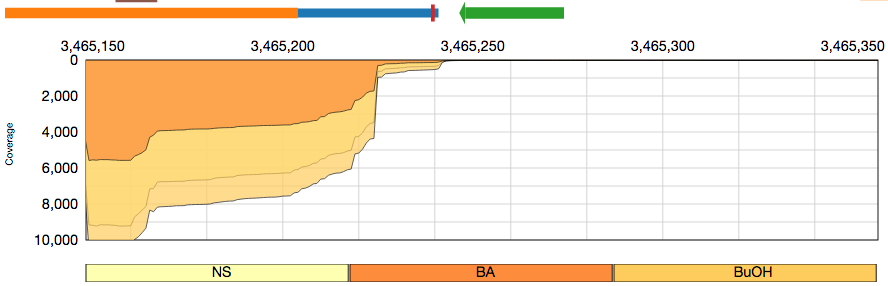
\includegraphics[width=\textwidth,height=1.5in]{images/Assembly/Examples/Bdh/BdhA-TSS.png}
\subcaption{BdhA Transcription Initiation Region}\label{fig:5a}}
{\includegraphics[width=\textwidth,height=1.5in]{images/Assembly/Examples/Bdh/BdhA-stop_site.png}
\subcaption{BdhA Transcription Termination Region}\label{fig:5b}}
{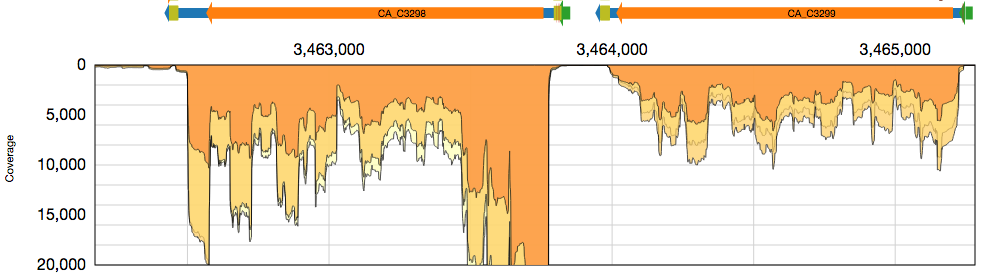
\includegraphics[width=\textwidth,height=1.5in]{images/Assembly/Examples/Bdh/Bdh-curated.png}
\subcaption{Curated BdhA Transcript}\label{fig:5c}}
\caption{Bdh Locus}
\subref{fig:5a}) The BdhA transcript displays a sharp increase in coverage near the transcriptional start site. This data agrees to a good extent with primer extension studies for this gene. \subref{fig:5b}) The raw assembly has failed to recapitulate the transcription termination region, likely due to low complexity coverage of the 3' region of this transcript. \subref{fig:5c}) The curated transcript reflects experimental characterization of this transcript\cite{72}.
\end{figure}

\paragraph{BdhB}
The next gene is BdhB, another NADH-dependent butanol dehydrogenase, with a slightly longer transcript size of 1.35kb. It was reported that this enzyme has 46-fold higher activity with butyryl groups than acetyl groups\cite{70,72}. BdhB was sequenced an analyzed along with BdhA, where it was discovered that BdhB had at least two transcription start sites, independent from BdhA. The most dominant transcription start site was very close to a secondary band at approximately 3,463,816 and 3,463,811, respectively\cite{72}. I will refer to these two distal bands collectively as the primary transcription start site for BdhB. A third band was located slightly farther upstream at 3,463,803\cite{72}. The coverage pattern for this region shows at least 3 sites of substantial increases in coverage at 3,463,802, 3,463,813, and 3,463,843 (\ref{fig:6a}). The first and proximal site has a promoter motif upstream, corresponding to the 1$^{st}$ -10 and -35 boxes in \ref{table:1} and the tertiary transcription start site\cite{72}. The second site has a significant increase in coverage between residue 3,463,817 and 3,463,810, which match well with the primary transcription start site described above\cite{72}. The primary transcription start site is explained by the 2$^{nd}$  -35 box and the 2$^{nd}$ or 3$^{rd}$ -10 box motifs\cite{72}. The final (distal) increase in coverage agrees with the 4$^{th}$ promoter motif(\ref{table:1}). It is clear that the strongest start site is the primary transcription start site previously described\cite{72}, although the multiple bands observed in their analysis could indeed be explained by matches to consensus Sigma-factor A motifs. Additionally, an observable but insignificant increase correlated with a final promoter motif. It is clear that the raw data match previous results to a good extent but curation was required to correct the transcription start site(\ref{fig:6a}) and stop site (\ref{fig:6b}). The final transcript is shown in \ref{fig:6c} with a final length of 1,367bp or 1,381bp, in close agreement with the published length of 1.35kb.

\begin{table}
\caption{BdhB Sigma-factor A boxes}\label{table:1}
\begin{minipage}[b]{2.5in}
\begin{center}
\begin{tabular}{|c|c|c|c|c|}\hline
\multicolumn{5}{c}{-35 box}\\\hline
Motif & Start & End & Sequence & p-value\\\hline
1 & 3463831 & 3463836 & TAGGTT & 3.5\e{-2}\\
2 & 3463847 & 3463852 & TTGTAA & 9.4\e{-3}\\
3 & 3463870 & 3463875 & TGGATA & 2.6\e{-2}\\\hline
\end{tabular}
\end{center}
\end{minipage}
\begin{minipage}[b]{2.5in}
\begin{center}
\begin{tabular}{|c|c|c|c|c|}\hline
\multicolumn{5}{c}{-10 Box}\\\hline
Motif & Start & End & Sequence & p-value\\\hline
1 & 3463816 & 3463821 & TATAAT & 4.3\e{-4}\\
2 & 3463820 & 3463825 & TATATA & 1.6\e{-3}\\
3 & 3463830 & 3463835 & TAAAAT & 4.2\e{-3}\\
4 & 3463852 & 3463857 & TATTAT & 4.2\e{-3}\\\hline

\end{tabular}
\end{center}
\end{minipage}
\end{table}
\begin{figure}
\small
{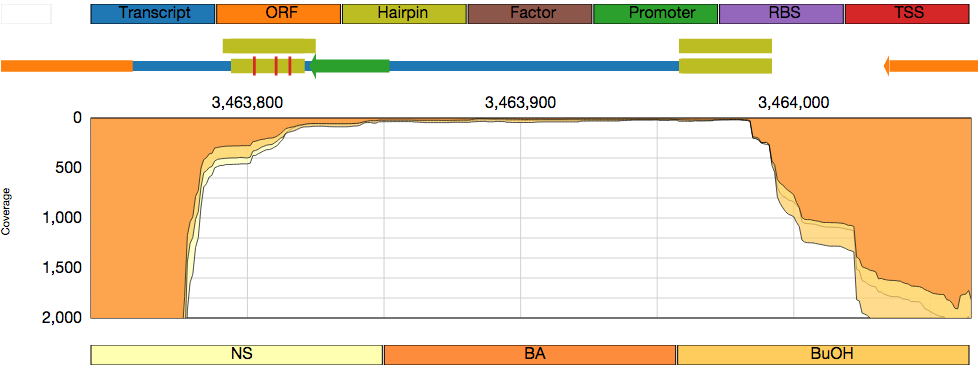
\includegraphics[width=\textwidth,height=1.5in]{images/Assembly/Examples/Bdh/BdhB-TSS.png}
\subcaption{BdhB Transcription Initiation Region}\label{fig:6a}}
{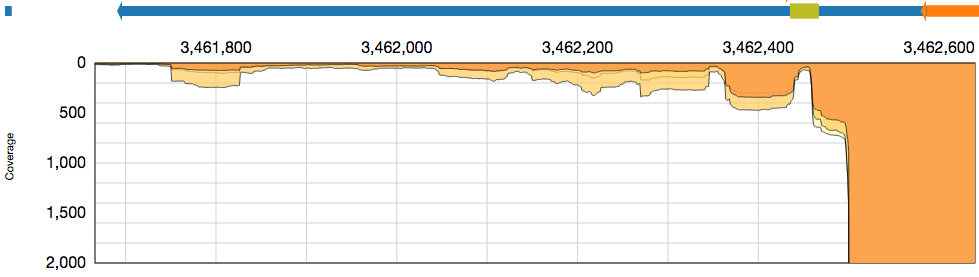
\includegraphics[width=\textwidth,height=1.5in]{images/Assembly/Examples/Bdh/BdhB-termination.png}
\subcaption{BdhB Transcription Termination Region}\label{fig:6b}}
{\includegraphics[width=\textwidth,height=1.5in]{images/Assembly/Examples/Bdh/BdhB-curated.png}
\subcaption{Curated BdhB Transcript}\label{fig:6c}}
\caption{Bdh Locus and Transcription Start Sites}
\subref{fig:6a}) The BdhB transcript has several promoter motifs and matching increases of coverage. These increases agree with previous experimental results\cite{72}, 2 of which were dismissed after not identifying the appropriate promoters. Unfortunately, the transcription start site was incorrect in the raw assembly. \subref{fig:6b}) A Rho-independent terminator is found at the end of the BdhB transcript although residual coverage triggered misassembly. \subref{fig:6c}) The final transcript matches previous results after integrating promoter and terminator motif information with the coverage pattern and assembly.
\end{figure}

In this example, the BdhA and BdhB transcripts were very close to capturing the true boundaries of these genes. In the case of BdhA the TSS was precise, but the assembled transcript did not match the coverage pattern or the ORF and terminator annotations. In the case of BdhB however, the start and stop sites did not agree with patterns in coverage and were simple to correct. The next example is another positive example, this time of a stress-response operon containing the heat-shock proteins GroES and GroEL.

\subsubsection{GroES/EL Locus}
\paragraph{GroES/EL Operon}
The GroES and GroEL proteins are evolutionarily conserved heat-shock responsive chaperonins. These proteins are found throughout the tree of life, including \textit{C. acetobutylicum}, where they are an integral to the solvent stress response\cite{73,74,75} and the class I heat-shock response\cite{42,73,74}. Expression levels are both strong and constitutive for this region, with a dramatic and transient increase with solvent or heat stress\cite{73,74}. In a molecular study, GroES and GroEL were found to be produced from a bicistronic operon with a transcript size of 2,150bp\cite{75}. In addition, a Sigma-factor A promoter was identified for an experimentally determined transcription start site. Two bands were observed during the primer-extension assay\cite{75}. The proximal band was dismissed as an artifact although the bands persisted under all conditions examined\cite{75}. This region is known to contain at least one CIRCE motif upstream\cite{76} and one overlaps both of these start sites (\ref{fig:7a})\cite{74}. The transcription start site determined in this work is located at 2,829,142, a mere two bases away from the previously reported start site\cite{75} (\ref{fig:7a}). Interestingly, the second transcription start site is located at a sharp increase in expression. The distance of this start site from the promoter suggests post-transcriptional processing. The transcription stop site is located near a Rho-independent terminator (\ref{fig:7b}). The transcript size determined by the raw assembly is 2,131bp in agreement with the 2.2kb band and the 2,150bp calculated distance between the transcription start-site and the Rho-independent terminator\cite{75}. In this example, the uncurated assembly produced a flawless recapitulation of the coordinates and size of the GroES/EL operon (\ref{fig:7b}). Having established the coordinates for this transcript in agreement with previous findings, the regulation of this operon should be briefly discussed.

\paragraph{GroES/EL Regulation}
The GroES/EL operon is stress responsive, although its expression under stress appears lower in \ref{fig:7c}. For this reason, it is worth discussing the regulation of this region and why these results are consistent with knowledge of this area. The CIRCE motif upstream of GroES is regulated by HrcA, a heat responsive repressor\cite{42,76,77}. In response to heat-shock, the GroES/EL operon is derepressed, revealing a Sigma factor A promoter and resulting in transcription (\ref{fig:7a}). The response to heat shock is fairly acute, increasing for 2-3 minutes and returning to standard levels after an additional 10 minutes\cite{76}. Here a general decreased expression is observed in response to solvent stress for two reasons. First, the 6S small RNA is a stress and growth-stage responsive regulator that globally reduces transcription from Sigma factor A promoters\cite{39,78}. Additionally, the time scale assessed here does not include a 3 minute time-point to identify an acute stress response. The stress response observed is the global downregulation of Sigma factor A promoters and the transition of the transcriptome towards one designed to tolerate stress. Sigma factor A dependent promoters are downregulated throughout this dataset as a result of the 6S small RNA. For this reason, we defer the test of differential expression for these time points for the next chapter. In the case of the GroES/EL operon, we observe precise and accurate estimates of transcript boundaries from the uncurated assembly. Additionally, we observe the effect of a complicating factor in differential analysis: the effect of the 6S small RNA on Sigma A dependent promoters at the time scales we are analyzing. The next example is the regulator responsible for the acute stress response of these heat shock proteins, HrcA.


\begin{figure}
\small
{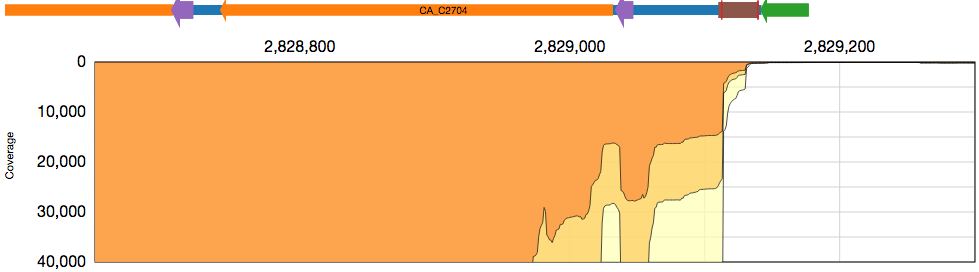
\includegraphics[width=\textwidth,height=1.5in]{images/Assembly/Examples/GroESL/GroESL-TSS.png}
\subcaption{GroES/EL Transcription Initiation Region}\label{fig:7a}}
{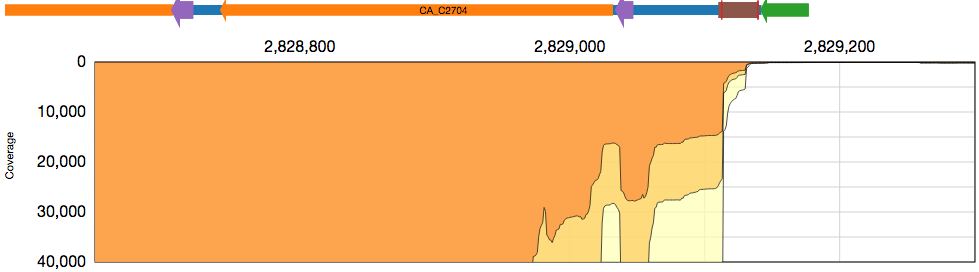
\includegraphics[width=\textwidth,height=1.5in]{images/Assembly/Examples/GroESL/GroESL-TSS.png}
\subcaption{GroES/EL Transcription Termination Region}\label{fig:7b}}
{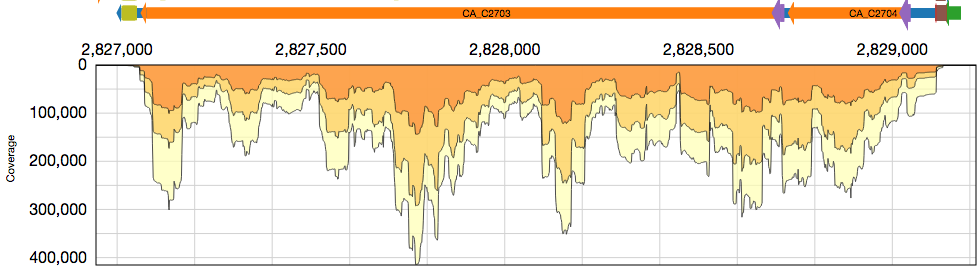
\includegraphics[width=\textwidth,height=1.5in]{images/Assembly/Examples/GroESL/GroESL-curated.png}
\subcaption{GroES/EL Locus}\label{fig:7c}}
\caption{GroES/EL Locus}
\subref{fig:5a}) GroES and GroEL form an operon that is responsive to heat-shock through a HrcA-mediated derepression mechanism. The transcription start sites are in agreement with previous findings with the addition of an interesting peak inbetween these two. \subref{fig:5b}) The transcription termination region supports previous reports of a 2.2kb transcript terminating at a Rho-independent terminator following the GroEL ORF.
\end{figure}

%   H r c A,  G r p E,  D n a K,  &  D n a J
\subsubsection{HrcA and DnaK/J Locus}
\paragraph{DnaK Locus Overview}
This rather complex locus encodes the class I repressor HrcA and DnaK and DnaJ, another set of evolutionarily conserved heat-shock proteins. DnaK was discovered to be solvent-stress responsive in \textit{C. acetobutylicum}\cite{73,74}. Solvent stress and heat shock increase protein denaturation, requiring molecular chaperones such as GroES/EL and DnaK/J to increase proper protein folding in these conditions. The \textit{C. acetobutylicum} DnaK protein was purified as a stress responsive 74kDa protein\cite{74}. Using a restriction fragment, the DnaK locus was then cloned and sequenced\cite{79}, revealing a grouping of four ORFs, similar in arrangement to \textit{B. subtilis}\cite{76}. An inverted repeat, now known to be the HrcA-binding CIRCE motif, was found upstream of the HrcA gene\cite{79}. Upon Northern analysis of this region, three different transcripts were identified as originating from this locus, of 2.6, 3.8, and 5kb lengths. Additionally, a 1.5kb band was observed with a DnaK specific probe\cite{79}. The first transcript (2.6kb) could be seen with a DnaK-specific probe and is thought to contain the genes GrpE and DnaK. The second transcript (3.6kb) was observed for both DnaK and HrcA-specific probes and is thought to contain the same genes plus HrcA. Similarly, the 5kb transcript was observed for both probes and is thought to contain the whole operon. The final transcript(1.4kb) and additional small bands were dismissed as specific degradation products. It has been noted that this operon has interesting post-transcriptional regulation in \textit{B. subtilis}, producing multiple transcripts from a heptacistronic operon\cite{82}. To analyze this complex operon, we will proceed through 4 proposed regulatory sites. The first is the promoter region of HrcA. The second site is a transcription start site upstream of GrpE. The third is the location of an internal CIRCE motif, terminator, and an additional transcription start site ahead of DnaJ. The final site is located at the end of the whole operon.

\paragraph{HrcA Promoter}
The HrcA promoter was described during the sequencing of the DnaK/J locus\cite{79}. This promoter produces the full transcript of 5kb and the smaller 3.6kb transcript terminating between DnaK and DnaJ. Two transcription start sites have been described for this region\cite{79}. Both of the two reported transcription start sites(S1 and S2) were located upstream of the CIRCE element, in contrast to groES/EL (\ref{fig:8a}). Additional bands present in the primer extension analysis were rejected similarly to the strand bands in the GroES/EL operon. An excellent Sigma factor A motif was located for the S1 site (P1,\ref{table:2}) but only an insignificant motif (p > 0.05, TTTATG(17)AAAGAT) motif was found for the weak band of the S2 site. An alternative promoter (P2, \ref{table:2}) seems to be too close to the S2 transcription start site. If the observed bands represent true transcription start sites for this operon they are transcribed from close and overlapping promoter motifs. Here we don't see any direct increase in transcription for the S1 site, most likely due sequencing difficulty near the CIRCE motif. Upon TEX enrichment, no increase or decrease in coverage can be observed near these sites, suggesting that post-transcriptional processing is not responsible for these transcription start sites. The increases in transcription observed here are relatively minor compared to the transcription of the entire HrcA operon. The P1 and P2 motifs seem to be sufficient for transcription initiation, although the coverage pattern shows evidence of complication of sequencing. In several studies\cite{75,79} transcription start sites have been discarded due to local RNA secondary structure. It is reasonable that reverse transcription in this area may be complicated by the -10kcal/mol hairpin and CIRCE motif near the 5' end of the transcript. Several authors have noted that full HrcA/DnaK operon transcripts are present at lower abundance\cite{79,82}, resulting in lower coverage and an indistinct transcription start site when considering coverage alone. In \ref{fig:8a}, it is clear that the uncurated assembly estimated the transcription start site more accurately than a coverage-only approach would provide. As we have seen, in some cases the De-bruijn graph assembly requires curation to most accurately reflect local motifs. On the other hand, this method produces a reasonable estimate of the start site. After minor curation, the transcription start site agrees with the previously described\cite{79} S2 and S1 (\ref{fig:8b}). Having established the transcription start site for the entire HrcA operon and previous transcriptional start sites are not the result of post-transcriptional processing, we move on to the higher abundance transcripts produced by this region, beginning with the GrpE operon.

\paragraph{GrpE Promoter}
The GrpE protein is an essential nucleotide exchange factor for DnaK. This protein was discovered upstream of DnaK after cloning and sequencing of the DnaK locus\cite{79}. It was postulated that a second transcription start site upstream of GrpE would explain the smaller transcripts described above and a transcription start site was determined\cite{79}. A transcription start site exists ahead of the GrpE gene in \textit{B. subtilis} as well\cite{82}. The proposed promoter ahead of GrpE does not match the Sigma factor A consensus (p > 0.05) and no alternative motifs were found. However, a substantial increase in coverage can be found further upstream from this site. The first two sites are specifically enriched in the TEX treated library, suggesting a transcription start site. Promoter motifs of higher quality are found upstream of two major peaks (\ref{fig:8b}). Looking at the entire operon (\ref{fig:8c}) it is clear that this is a substantial transcription start site. 

\begin{figure}
{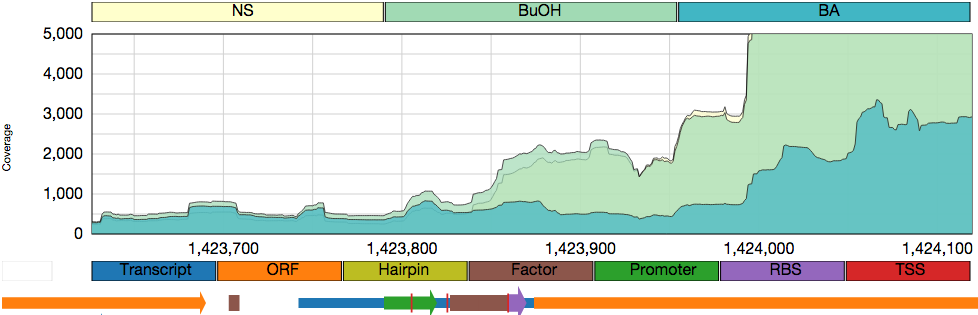
\includegraphics[width=\textwidth,height=1.5in]{images/Assembly/Examples/HrcA/HrcA-TSS.png}
\subcaption{HrcA Transcription Initiation Region}\label{fig:8a}}
{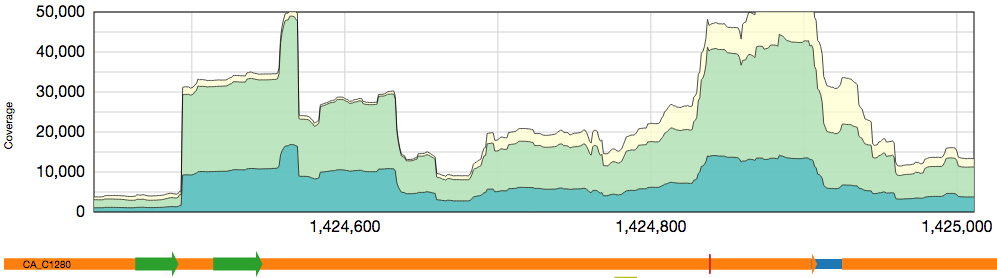
\includegraphics[width=\textwidth,height=1.5in]{images/Assembly/Examples/HrcA/GrpE-TSS.png}
\subcaption{GrpE Transcription Initiation Region}\label{fig:8b}}
{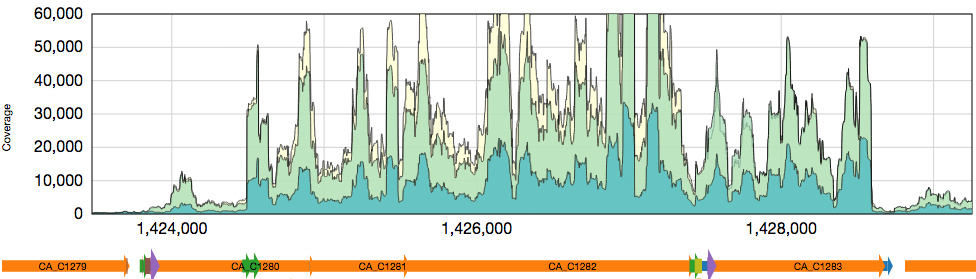
\includegraphics[width=\textwidth,height=1.5in]{images/Assembly/Examples/HrcA/HrcA-operon-curated.png}
\subcaption{Curate HrcA Locus}\label{fig:8c}}
\caption{HrcA Locus}
\subref{fig:8a}) HrcA leads the 5kb tetracistronic operon. The regulation of this operon consists of Sigma factor A dependent promoters, a CstR motif, and a CIRCE motif. \subref{fig:8b}) A secondary transcription start site in upstream of GrpE is responsible for the 2.6kb and 3.8kb transcripts. The previously reported proximal TSS is shown with a large increase in coverage at a novel distal transcription start site. \subref{fig:8c}) The curated HrcA operon has two transcription start sites and one Rho-independent terminator which explain the 5kb, 3.8kb, and 2.6kb transcipts reported for this area.
\end{figure}


\begin{table}
\caption{HrcA Operon Sigma-factor A boxes}\label{table:2}
\begin{minipage}[b]{2.5in}
\begin{center}
\begin{tabular}{|c|c|c|c|c|}\hline
\multicolumn{5}{c}{-35 box}\\\hline
Motif & Start & End & Sequence & p-value\\\hline
P1 & 1423790 & 1423795 & TTGACA & 2.9\e{-4}\\
P2 & 1423774 & 1423779 & ATGAAA & 5.3\e{-2}\\
P3 & 1424463 & 1424468 & TTGAGG & 1.6\e{-2}\\
P4 & 1424514 & 1424519 & TTGATT & 6.2\e{-3}\\
\hline
\end{tabular}
\end{center}
\end{minipage}
\begin{minipage}[b]{2.5in}
\begin{center}
\begin{tabular}{|c|c|c|c|c|}\hline
\multicolumn{5}{c}{-10 Box}\\\hline
Motif & Start & End & Sequence & p-value\\\hline
P1 & 1423812 & 1423817 & TATTTT & 2.3\e{-2}\\
P2 & 1423800 & 1423805 & TAATGT & 1.8\e{-2}\\
P3.1 & 1424476 & 1424481 & TAATAT & 9.9\e{-3}\\
P3.2 & 1424482 & 1424487 & TAAAAA & 3.2\e{-2}\\
P4 & 1424537 & 1424542 & TATGAT & 1.9\e{-3}\\

\hline
\end{tabular}
\end{center}
\end{minipage}
\end{table}

\paragraph{DnaK/J Intergenic Region}



In this dataset, the coverage pattern matches very well with the previously published transcript size of 5kb. Interestingly, the HrcA transcription start site determined by the uncurated assembly is comparable to previous studies. Moreover, the assembly predicts a transcription start site with reasonable accuracy, considering the level of residual signal from the upstream gene. The data could certainly reflect the transcriptional terminator downstream of DnaK, but no Rho-independent terminator was found downstream of DnaJ using three different algorithms. The termination of this transcript may be due to a non-intrinsic termination mechanism. This region has also been fused to signal from the downstream gene.

\begin{figure}
\small
{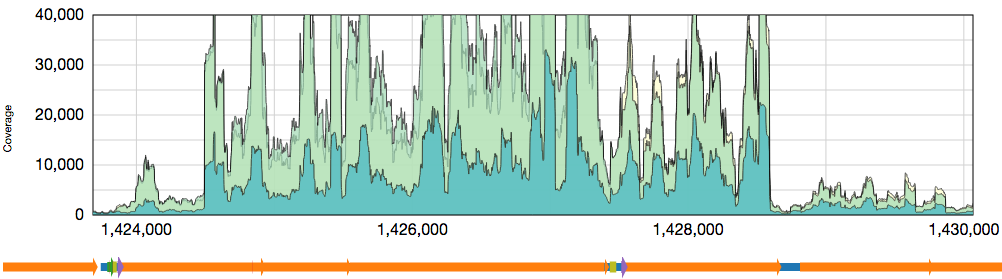
\includegraphics[width=\textwidth,height=1.5in]{images/Assembly/Examples/HrcA/HrcA-locus.png}
\subcaption{Operon consisting of HrcA, GrpE, DnaK, and DnaJ}\label{fig:7a}}
{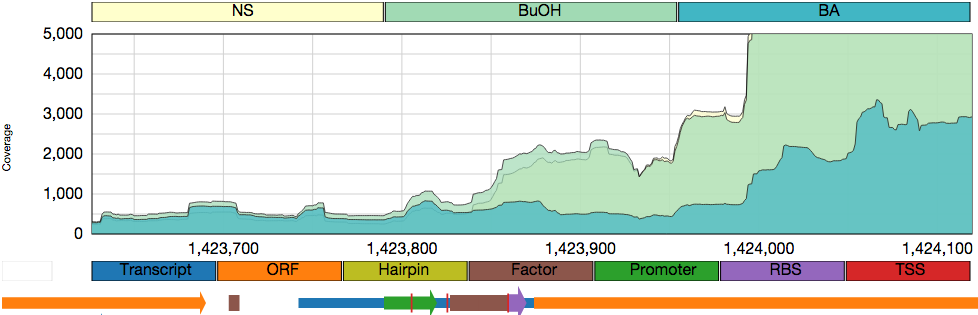
\includegraphics[width=\textwidth,height=1.5in]{images/Assembly/Examples/HrcA/HrcA-TSS.png}
\subcaption{HrcA transcription initiation region.}\label{fig:7b}}
{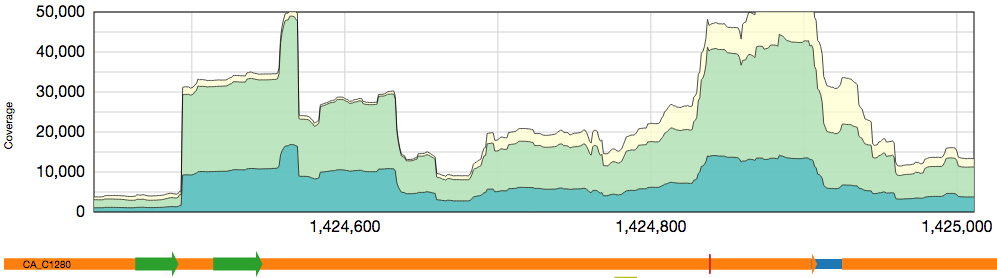
\includegraphics[width=\textwidth,height=1.5in]{images/Assembly/Examples/HrcA/GrpE-TSS.png}
\subcaption{GrpE transcription initiation region.}\label{fig:7c}}
{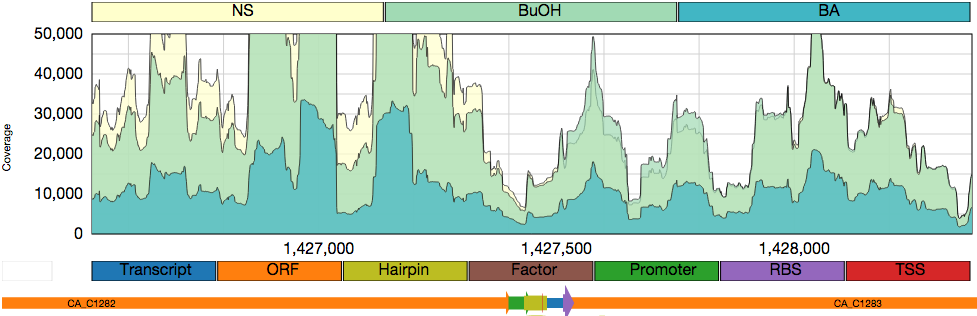
\includegraphics[width=\textwidth,height=1.5in]{images/Assembly/Examples/HrcA/DnaKJ-IGR.png}
\subcaption{DnaK-DnaJ IGR and DnaJ transcription initiation region}\label{fig:7d}}
\caption{HrcA locus}
\subref{fig:7a}) The highly expressed HrcA locus encodes several transcripts of different size. \subref{fig:7b}) The assembled transcription start site for the HrcA gene provides a reasonable estimate, considering the level of background signal for this region. \subref{fig:7c}) The transcription start site is not distinguishable in the coverage data. \subref{fig:7d}) The intergenic region between DnaK and DnaJ contains the only hairpin for this operon, which matches a decrease in coverage. The reported transcription start site is not identifiable from the coverage in this region.
\end{figure}

%          S p o 0 A

Spo0A is the master regulator of sporulation and stationary phase phenomena. This protein is thought to ultimately transduce growth-limiting and stressful signals into sporulation behavior in a number of anaerobic firmicutes. In previous studies, Spo0A was shown to be translated from a 0.9kb transcript in \textit{C. acetobutylicum}. Here we observe a slightly longer transcript of ~1.1kb according to the pattern of coverage. However, no Rho-independent terminators were found immediately downstream (\textless  200bp) of Spo0A, suggesting either a non-intrinsic termination mechanism or differing transcript sizes from those previously reported. Unfortunately, the boundaries represented by this coverage pattern were not detected due to the background signal in the area. Consequently, this region needs some remediation and is the first example of a completely fused transcript, not merely an extension.

In a nearby location, the genes CAC2073-2078 are found in a tight grouping near a large peak of expression. This peak correpsonds to an uncharacterized protein CAC2079 that is present in UniProt but absent from NCBI and KEGG databases. Its coverage appears to be largely above 20k per base, independent of the surrounding regions (although the transcript is indeed fused). Bioinformatic analysis suggests that it shares sequence similarity to proteins in the \textit{Clostridia}, \textit{Bacilli}, \textit{Baceteroidetes}, and \textit{Halobacteria}. While there was no common catalytic or active domain unifying this group of homologs, the region of homology tends to precede a transmembrane motif. Further analysis via PSI-blast result suggests sequence similarity to mATE (Multidrug And Toxic-compound Extrusion) efflux family proteins. mATE family proteins use electrochemical gradients to export antibiotics and other toxic compounds. The data suggest that the expression of this protein is important to \textit{C. acetobutylicum} and it will be interesting to examine the expression profile statistically. This instance demonstrates the synergy of older annotations with the newer coverage data and once again the need for semi-automated curation. Next we explore another stress-responsive region with a regulatory protein, the HrcA locus.

\begin{figure}
\small
{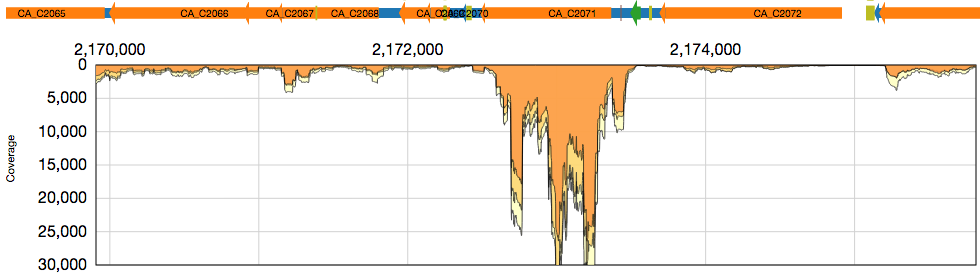
\includegraphics[width=\textwidth,height=1.5in]{images/Assembly/Examples/Spo0A/Spo0A-locus.png}
\subcaption{Spo0A transcript (center) fused to signal from neighboring regions}\label{fig:6a}}
{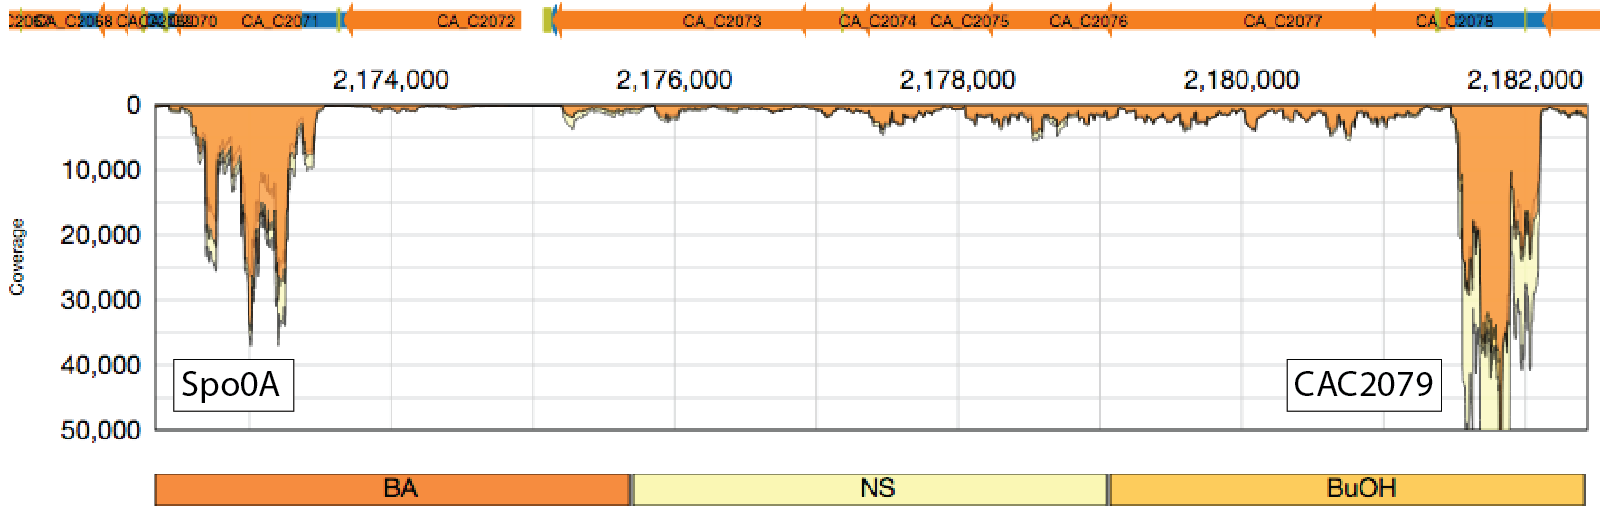
\includegraphics[width=\textwidth]{images/Assembly/Examples/Spo0A/CAC2079.png}
\subcaption{Upstream region of Spo0A, including CAC2079, a putative protein missing from many databases.}\label{fig:6b}}

\caption{Spo0A locus}
\subref{fig:6a}) The Spo0A transcript is found in a region of sufficient k-mer complexity and background coverage for the assembled transcript to be fused to signal from neighboring operons. This region clearly requires attention from curation strategies. \subref{fig:6b}) The region upstream of Spo0A consists of a late stage sporulation protein and a group of proteins in tight formation. Interestingly, there is a missing annotation in NCBI and KEGG for protein CAC2079 near a large peak of expression, in between the annotated proteins CAC2078 CAC2080.
\end{figure}


\subsection{Identify and Attempt to Resolve Remaining Issues}
There are two principal challenges relating to this uncurated transcriptome assembly. The first relates to the qualification of novel transcripts which I will defer to a later time. The second involves the curation of the 1057 transcripts which encode reference CDSes. After considering the examples above, we are left with a few types of misassembly to address.
\begin{enumerate}
\item Partial transcripts which overlap reference ORFs, but do not completely contain them. (e.g. BdhA)
\item Extended transcripts that possess larger UTRs than would be expected with respect to promoter and terminator motifs and coverage patterns. (e.g. Adc, CtfA/B)
\item Fused transcripts where the transcript from one gene is completely fused with signal from neighboring loci, with respect to prior knowledge, promoter, and terminator motifs (e.g. Spo0A).
\end{enumerate}

The first issue requires the simple solution of adjusting the transcript boundaries to include reference ORFs where there is not complete inclusion. Practically this requires only some minimal scripting and the use of '\href{http://bedtools.readthedocs.org/en/latest/content/tools/merge.html}{merge}' from bedtools, a toolkit for genomic set operations. The second issue requires a slightly more complicated solution of integrating information of regulatory motifs, terminators, and coverage information to find the solution that produces the most agreement between these various sources. In practice, I will integrate the various sources in the genome browser for context with the coverage information from this experiment. No completely automated tools exist to accomplish this. However, on average each transcript requires only a minimal amount of decision and should in principle be easy to curate. The third type of gene is completely fused to signal from other genes or noise. In the case of Spo0A, the true signal was simple to distinguish from noise, even in the absence of a Rho-independent terminator. In other cases the solution may not be so simple but contextual information about ontology combined with the various signals of coverage and stress response, promoters, and terminators make the problem more tractable. 

In principle, each of the pieces of information that I will integrate will not reproduce the transcript boundary on its own. In the examples above there are instances where the coverage alone fails to describe the transcript boundary, while the linguistic complexity of the dataset, used by the assembly algorithm, reproduces the boundary to a good extent. In other instances the opposite is true: a dramatic change in coverage near terminators or other signals is not recognized by the assembly alone. For that matter, there appear to be instances of non-intrinsic termination to complicate matters further. Therefore, these information are synergistic with respect to defining transcript boundaries and the absence of one signal may be made up for by the presence of another.

\subsection{Novel Transcripts}

\subsection{Exploratory Tools}


    % These files contain the results sections
% This is the Chapter 4 - Differential expression and supplemental analyses

\chapter{Differential Expression}



%					C H A P T E R   5 - Discussion
% This is the Chapter 4 - Discussion file (discussion.tex)

\chapter{Discussion}

    % This file (discussion.tex) contains the text
                   % for Chapter 4- discussion

%					C H A P T E R   6 - Conclusions


% This is the Chapter 5 - Conclusions file (conclusions.tex)

\chapter{Conclusions}

Renewables research revolves around the development of a feedstock-flexible chassis organism that requires minimal engineering for biofuels production, such as \textit{C. acetobutylicum}. The development of this organism requires a complete genome annotation consisting of ORFs, promoters, terminators, and transcript boundaries. The existing annotation of this microbe is largely the result of ORF predictions from antiquated gene models and is consequently incomplete. Genomic and molecular research will be more efficacious with an accurate genome annotation.

High-throughput transcriptomic methods such as RNA-seq are ideal to update this annotation, despite the well documented challenges related to this platform. Many of these challenges have not been addressed by the literature, leading to poor data utilization rates(Table \ref{table:study_compare}). The absence of standards for bacterial transcriptome mapping studies provided the opportunity to develop an innovative technique to explicitly address false positive and false negative signal in sequencing datasets.

Several problematic issues, including rRNA and RNA degradation, were addressed by developing a laboratory workflow and quality control system prior to deep sequencing. The dataset was cleaned for errors, biases, and contaminants for proper quantification of the sensitivity. 450M properly-paired reads provided \textgreater 9000 fold-coverage of the \textit{C. acetobutylicum}, with a median per-base sequencing depth of 156x. This method even detected low-level background signals, an issue affecting deep sequencing studies that leads to false positive errors, yet ignored by studies in the microbial community. 

To identify and treat these issues, a fast and flexible genome browser was constructed. The genome browser visualized the background signals and misassemblies that were detectable in assembly statistics. Genome-wide promoter predictions revealed the prevalence of $\sigma_{A}$-promoter elements in the AT-rich \textit{C. acetobutylicum} genome, a potential source for the background signals. An integrative analysis method was developed to correct the misassemblies where necessary by including sequencing depth, complexity, Rho-independent terminators, and promoter motifs in the annotation visualization and curation method.

Most examples required little to no curation and showed excellent precision and accuracy with respect to previous studies. Even challenging edge cases involving multiple transcription start sites had excellent signal to noise ratio and consequently simple corrections. A proof-of-principle curation of the pSOL1 megaplasmid produced ideal assembly statistics, including a median transcript size of 1.4kb consistent with the reported average transcript lengths in \textit{E. coli}. A total of 86 reference-ORF containing transcripts and 24 novel transcripts were identified.

By explicitly addressing several issues related to false positive and false negative signals, a sequencing protocol and integrative analysis method was developed. This method lead to the first strand-specific transcriptome assembly in the genus \textit{Clostridia}. The technique described by this work is applicable in any bacterial species where a genome sequence is available. While the unprecedented sequencing depth of this study lead to false positive results in the initial assembly, the integrative curation method provided both precision and accuracy in transcript boundary determination. 

\chapter{Future Work}
This study provided \textit{C. acetobutylicum} transcript boundaries for future molecular and genomics studies. The method used in the proof of principle curation of the pSOL1 megaplasmid should be extended to the entire \textit{C. acetobutylicum} chromosome. It is reasonable to expect that the transcript and UTR sizes for the whole genome should be similarly improved. The transcript boundaries could improve expression estimates and differential expression analyses. Beyond comparing with previous microarray studies, novel transcripts discovered here could be discovered to be stress responsive. Such findings would be natural targets for future targeted or whole genome stress response analyses. 

The transcript boundaries also facilitate regulatory motif identification. Besides the promoter motifs and transcription factor binding sites described here, new motifs could exist upstream of transcription start sites of clusters of co-regulated genes. Differential promoter usage can be investigated using the genome browser and gene-specific techniques. Gene networks in \textit{C. acetobutylicum} inevitably possess transcription activation systems and will be ready to be explored with a complete genome annotation.

In fact, differential expression and motif analyses can be combined in an interesting way. By coupling differentially expressed genes, their expression profiles, and clustering algorithms, patterns of co-expression and perhaps co-regulation may be identified. The performance of such an approach naturally depends on normalization approaches (to make profiles reasonably comparable) and clustering theory. While some approaches have been suggested for expression profiles specifically, the performance of any approach is ultimately determined by these two factors and thus all options should be explored. 

Additional research can be done with comparative genomics, including re-annotation of the genome and transcriptome for protein coding ORFs. With the example of the missing CAC2079 gene for example, there may be substantially transcribed and protein coding regions that require comparative analysis to identify metabolite exporters, two-component systems, and more. In fact, the RAST annotation system\cite{160} can be used to annotate transcriptomes, with some clever scripting and knowledge of its features.

Finally, additional analyses should be done for RNA hybridization and small RNA target prediction. Many recently identified stress responsive small RNAs\cite{39} have unknown targets and functions. Exploration of their roles has been prohibited by undefined UTR structures and thus the thermodynamics of interaction with their partners. A complete genome annotation provides these information and an additional tractable problem for \textit{C. acetobutylicum} researchers to explore.

The first assembly and annotation provided by this work presents a number of opportunities for additional work in \textit{C. acetobutylicum}. Increasing temperatures, CO$_{2}$ levels, and energy prices provide ethical and economical incentives to explore renewables research in this organism. A small number of intrinsic conditions have explored in this study, including the exponential and transition stages of growth, and stress responses to metabolite stress. Additional conditions may display alternate gene sets, expanding the complexity of the transcriptome beyond what is described here. Novel transcripts identified in the megaplasmid and chromosome require annotation and molecular study. If enzymes are discovered, metabolic models should be updated. Differential expression experiments are an increasingly useful method for understanding transcriptomic dynamics. Such studies in \textit{C. acetobutylicum} directly benefit from a wider and more complete genome annotation. This work facilitates future research in \textit{C. acetobutylicum} through the genome browser, which can incorporate future annotations and display expression data in a fast, flexible, and data-dense manner.



    % This file (conclusions.tex) contains the text
                   % for Chapter 6- conclusions


%					R E F E R E N C E S
%%
% This is the References file (ref.tex)
%
\renewcommand{\bibname}{References}
\begin{thereferences}
Lastname, Firstname  ``Title.''  \textit{Journal}, Year.

Lastname, Firstname, and Firstname Lastname.  \textit{Title of Book}.  Publisher, Year.
\end{thereferences}
      % This file (ref.tex) contains the text
                   % for the references.
                   
%%
% This is the Bibliography file (bib.tex)
%
% For 100-999 change 99 to 999; for 1000-9999 change 99 to 9999 
\begin{thebibliography}{99}
\bibitem{1}Lastname, Firstname  ``Title.''  \textit{Journal}, Year.

\bibitem{2}Lastname, Firstname, and Firstname Lastname.  \textit{Title of Book}.  Publisher, Year.
\end{thebibliography}
      % This file (bib.tex) contains the text
                   % for a bibliography.
                                      
%
% This is the Bibliography file (bibtex.tex)
% This generally works for BibTeX

% Use sample.bib for BibTeX database
%\phantomsection
%\addcontentsline{toc}{chapter}{ }
\renewcommand{\bibname}{BIBLIOGRAPHY}

\nocite{*}
\bibliography{endnote}{}
% BibTeX style (plain, alpha, unsrt)
\bibliographystyle{unsrt}



% N O T E: Make sure to convert back to endnote for Terry	 % This file (bibtex.tex) contains the text
                   % for a bibliography if using BibTeX with
                   % sample.bib
                                      
%%
% This is one Appendix file (app.tex)
%
\oneappendix{Title for Appendix}

This is the information for one appendix. This is to be used if there is only one appendix.      % This file (app.tex) contains the text
                   % for one Appendix. 

%			A P P E N D I X      A
%%
% This is the Appendix A file (appA.tex)
%
\appendix{Title of Appendix}

This is the information for the first appendix, Appendix A. Copy the base file, appA.tex, for each additional appendix needed such as appB.tex, appC.tex, etc. Modify the main base file to include each additional appendix file.

If there is only one appendix, then modify the main file to only use app.tex instead of appA.tex.     % This file (appA.tex) contains the text
                   % for Appendix A. 
 
 %			A P P E N D I X      B
%\include{appB}     % This file (appB.tex) contains the text
                   % for Appendix B.   
       
\end{document}